\chapter[基于分层车联网架构的车载信息物理融合质量指标设计与优化]{基于分层车联网架构的车载信息物理融合质量指标\\设计与优化}
本章将研究基于分层车联网架构的车载信息物理融合系统质量指标设计与优化。
本章内容安排如下:
\ref{section 2-1} 节是本章的引言,介绍了车联网服务架构与车载信息物理融合系统质量指标的研究现状、目前研究的不足,以及本章的主要贡献。
\ref{section 2-2} 节阐述了分层车联网架构设计。
\ref{section 2-3} 节介绍了分布式感知与异质信息融合场景。
\ref{section 2-4} 节设计了车载信息物理融合质量指标并形式化定义VCPS质量优化问题。
\ref{section 2-5} 节提出了基于差分奖励的多智能体强化学习算法用以优化VCPS质量。
\ref{section 2-6} 节搭建了仿真实验模型并进行了性能验证。
\ref{section 2-7} 节总结了本章的研究工作。

\section{引言}\label{section 2-1}

随着无线通信技术的蓬勃发展,车联网正逐步成为支持下一代智能交通系统的关键技术。随着 C-V2X 通信、大数据和人工智能的发展,汽车行业的下一场革命即将到来。回顾过去十余年手机的发展历程,可以看到手机已经从传统的通话和信息传递工具转变为具有社交、导航、多媒体娱乐等诸多功能的智能设备。类似于手机的发展,汽车不再仅是单纯的运输工具,而且将朝着智能化、网联化、协同化方向演进,成为支撑各种智能交通系统应用的关键。软件定义网络\cite{li2021zhi}和移动边缘计算\cite{liu2022fedcpf}新兴范式的涌现,为车联网提供了支持高密度车辆通信、海量数据传输、自适应计算卸载,以及逻辑集中控制等功能的解决方案。传感技术和车联网的最新进展也推动了车载信息物理融合系统的发展,并进一步推动下一代智能交通系统的实现。在VCPS中,交通灯信号、车辆位置、点云数据和监控视频等异质信息可以被车辆分布式感知并上传至边缘节点。边缘节点基于车辆感知信息进行融合,构建反映车联网中各元素的物理状态的逻辑映射,其被称为逻辑视图。因此,本章致力于提出一种新颖的分层车联网服务架构,以最大化软件定义网络和移动边缘计算范式的协同效应,并支撑实时、可靠的车载信息物理融合系统。在此基础上,考虑了车载分布式感知与异质信息融合场景,设计了车载信息物理融合质量指标与相应的调度算法,以最大化车载信息物理融合质量。

研究人员对车联网服务架构进行了深入研究。自2016年Liu等人\cite{liu2016cooperative}首次将SDN应用于车联网以来,大量研究人员围绕软件定义车联网进行了研究\cite{dai2018cooperative, luo2018sdnmac, liu2018coding, zhang2022ac-sdvn, zhao2022elite, lin2023alps, ahmed2023deep}。然而,现有的大部分工作仅仅是在软件定义车联网架构的基础上,从数据分发、路由缓存、数据安全等方面展开了研究,并没有对整体架构进行深入分析。另一方面,越来越多的研究在车联网环境中考虑将移动边缘计算范式应用于系统,以提高实时性、可靠性和安全性\cite{liu2017a, lang2022cooperative, liu2021fog, dai2021edge, zhang2022digital, liu2020adaptive, liao2021learning, liu2023mobility, liu2023asynchronous}。然而,上述研究并没有考虑在异构车联网中最大化不同服务架构的协同效应。研究人员围绕车联网中的数据传播 \cite{liu2021fog, singh2020intent}、信息缓存 \cite{zhang2022digital, dai2020deep, su2018an} 和任务卸载 \cite{shang2021deep, liao2021learning} 方面展开了深入研究。然而,现有研究工作都没有考虑分布式感知和异质信息融合的协同效应。部分研究人员对VCPS中的预测 \cite{zhang2019a, zhang2020data}、调度 \cite{li2020cyber, lian2021cyber} 和控制 \cite{dai2016a, hu2017cyber, lv2018driving}技术进行了大量的研究,并促进了各种ITS应用的实现。然而,上述研究都是基于边缘/云节点能够收集足够且可靠信息的基础上。部分研究聚焦于VCPS中的信息质量评估\cite{liu2014temporal, dai2019temporal, liu2014scheduling, rager2017scalability, yoon2021performance}。然而,大部分研究工作只评估了数据项层面的质量,而忽略了对异质信息融合的质量评估。部分研究专注于车联网中使用深度强化学习的车辆传感和信息融合\cite{dong2020spatio, zhao2020social, mlika2022deep},但并不适用于多车场景。少数研究将多智能体DRL应用于车联网中\cite{kumar2022multi, he2021efficient}。然而,这些解决方案都不能直接应用于车载信息物理融合系统中的分布式感知和异质信息融合。

基于以上分析,本章针对分层架构和质量指标进行了协同研究,在分层车联网架构基础上实现分布式感知和异质信息融合,并提高车载信息物理融合质量。本章的主要贡献如下:第一,提出了融合软件定义网络和移动边缘计算范式的车联网分层服务架构。该架构包含应用层、控制层、虚拟层和数据层,通过分离车联网中控制和数据平面实现了逻辑集中控制,并通过卸载边缘的网络、计算、存储资源实现了基于MEC的分布式服务。第二,提出了分布式感知与异质信息融合的场景,并建立了基于多类M/G/1优先级队列的分布式感知模型。在此基础上,设计了一个名为Age of View (AoV) 的车载信息物理融合质量指标,用于评估VCPS中异质信息的时效性、完整性和一致性。进一步,形式化定义了车载信息物理融合质量最大化问题。第三,提出了一个基于差分奖励的多智能体深度强化学习(Multi-Agent Difference-Reward-based Deep Reinforcement Learning, MADR)算法来最大化VCPS质量。具体地,车辆作为独立的智能体,其动作空间包含感知频率和上传优先级。然后,设计了一个基于差分奖励(Difference Reward, DR)的信用分配方案来评估各个车辆对视图构建的贡献,从而提高每个智能体行动的评估精度。同时,设计了一个基于车辆预测轨迹和视图需求的V2I带宽分配(V2I Bandwidth Allocation, VBA)方案。第四,基于现实世界的车辆轨迹,构建了仿真实验模型,并进行了全面的性能评估。具体地,实现了所提 MADR 算法和 4 种比较算法,其中包括随机分配(Random Allocation, RA)、集中式深度确定性策略梯度(Centralized Deep Deterministic Policy Gradient,C-DDPG)\cite{mlika2022deep}、多智能体行动者-评论家\cite{he2021efficient}和采用VBA策略的多智能体行动者-评论家(Multi-Agent Actor-Critic with V2I Bandwidth Allocation, MAAC-VBA)。仿真结果表明,与C-DDPG、MAAC和MAAC-VBA相比,MADR 算法在提高VCPS质量方面分别高出约61.8\%、23.8\%、22.0\%和8.0\%,收敛速度分别加快了约6.8倍、1.4倍和1.3倍。

\section{分层车联网架构设计}\label{section 2-2}

为了改造和革新传统网络架构,研究人员提出了软件定义网络\cite{wang2020ji},其实现逻辑上的集中控制和网络功能快速迭代。目前,SDN 在云计算系统中的控制和管理已经显现出了巨大优势\cite{jain2013network}。其核心思想是通过解耦网络中的控制平面和数据平面来简化管理,加速网络系统的演进。在控制平面,网络中的控制功能集中于 SDN 控制器,并通过基于软件的方式实时修改和更新网络传输规则。在数据平面,网络节点(如交换机)将根据 SDN 控制器的决策转发数据包。然而,车联网的快速发展给传统的车联网架构带来了诸多挑战。例如,由于传统网络架构中网络控制和数据转发功能耦合,难以满足车联网中时变网络需求,并满足车联网实时性、可靠性和安全性等性能需求。SDN将网络控制和数据转发的功能解耦,实现网络资源的灵活配置和优化。具体地,SDN控制器位于云端,实现对车联网中所有的流量进行集中控制。此外,SDN的虚拟化技术可以将车联网中的物理资源虚拟化,使得网络资源管理更为高效和灵活。基于SDN技术,车联网可以实现更加精细化的管理和调度,提高网络的可靠性和性能,为智能交通系统应用提供更好的支持。考虑到车联网中动态网络拓扑、车辆高移动性和异质通信接口等特点,亟需一个基于 SDN 的框架来抽象资源,并在该系统中实现最佳服务调度。

另一方面,移动边缘计算能够在物联网时代为数十亿联网设备提供高可靠性和低延迟的信息服务 \cite{shi2016edge}。MEC通过将计算、网络、存储资源从云端卸载到终端用户附近,从而有效地缩短数据传输和响应时间,提高服务的可靠性和响应速度。与传统基于云的服务不同,MEC专注于支持高密度的设备连接和网络边缘的密集计算。毋庸置疑,车联网作为物联网中最具代表性的应用场景之一,有望从基于边缘的服务发展中获得巨大的收益。车联网不仅代表着车辆之间的连接,更重要的是,它还代表着行人、道路、基础设施等之间的协作。通过MEC技术,车联网能够实现实时数据采集、处理和传输,使车辆之间的协作更加高效和精确。同时,MEC还可以通过在车辆和设施之间构建更加紧密的联系,实现更加智能的交通控制,从而提高交通安全和效率。值得注意的是,5G技术的成熟和现代汽车在计算、存储和通信能力方面的快速发展,正强力驱动着MEC与车联网的结合 \cite{li2021che}。超可靠和低延迟的5G技术可以大幅提高数据传输和响应速度,进一步提升车联网的效率和可靠性。而现代汽车的智能化趋势也为移动边缘计算的应用提供了更为广泛的可能性。

本章提出了一个新颖的车联网分层架构,旨在增强信息服务的可扩展性和可靠性,提高应用管理的敏捷性和灵活性,并为下一代 ITS 的实现奠定坚实的基础。如图 \ref{fig 2-1} 所示,该架构一共具有四层:应用层、控制层、虚拟层和数据层。具体地,该架构的最上层是面向业务需求的应用层,其中包括安全认证、交通管理、数据管理等各种ITS应用。控制层负责管理和控制网络资源,而虚拟层用于虚拟化和管理网络、计算和存储资源。位于底层的数据层负责存储和处理车联网产生的各种数据,以支持上层应用。本架构的设计整合了SDN和MEC范式,以最大限度地利用它们对车联网信息服务的协同效应。其主要目标包括:a)在高动态车联网环境中实现逻辑上的集中控制;b)在异构车联网环境中实现网络功能虚拟化,并为具有不同QoS要求的服务实现网络切片;c)协调基于云和边缘的服务,最大限度地利用车联网中的网络、计算、通信和存储资源。

\begin{figure}[h] 
	\centering
	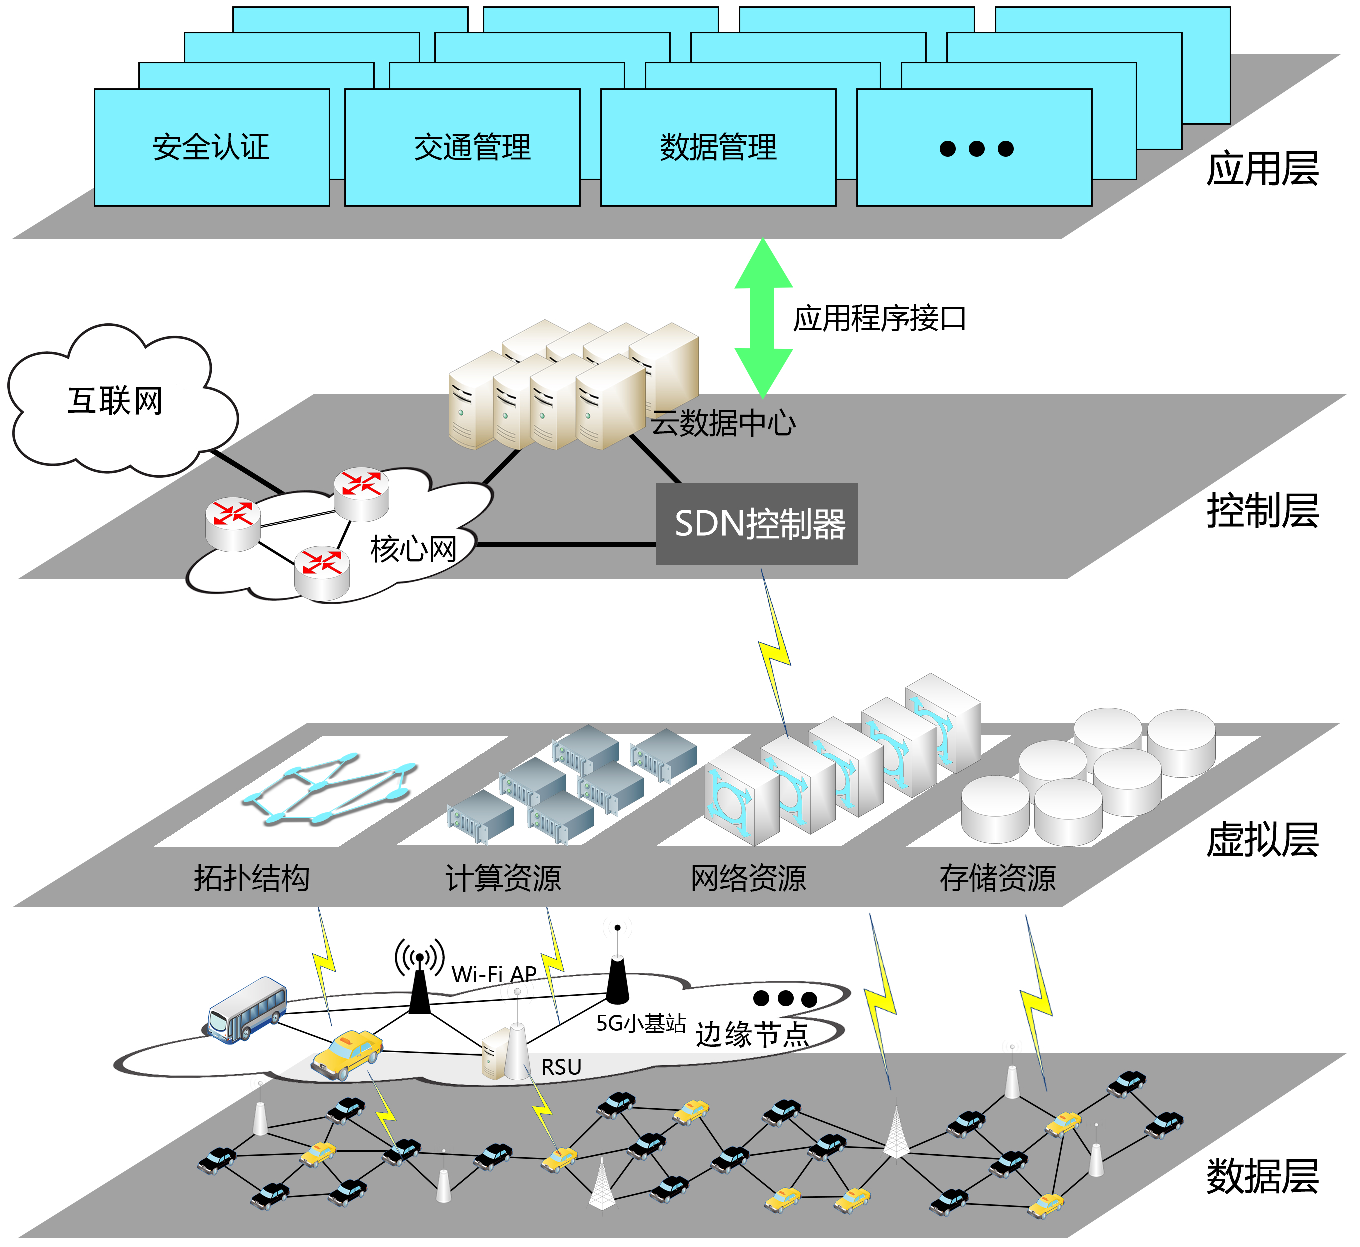
\includegraphics[width=1\columnwidth]{Fig2-1-hierarchical-architecture.pdf}
	\bicaption{异构车联网分层服务架构}{Hierarchical architecture for heterogenous vehicular networks}
	\label{fig 2-1}
\end{figure}

\subsection{基于移动边缘计算的车联网分布式服务}

本架构的数据层由如LTE基站、RSU、Wi-Fi接入点(Access Point, AP)、5G小基站和车辆等数据节点组成。除了不同的无线通信接入能力,数据节点还具备一定的计算和存储能力。其中,一些节点被抽象为边缘节点用于提供分布式服务。移动和静态的数据节点可以根据调度服务的需要被动态地分配为边缘节点。特定车辆如公交车和出租车等也可作为移动边缘节点。边缘节点不仅可以根据SDN控制器的规则执行操作,还可以为本地服务实现某些智能,进一步提高服务质量和效率。同时,边缘节点对底层资源进行一定的聚合和抽象,并向虚拟层实时更新状态,从而有助于虚拟资源的管理。因此,SDN控制器可以更方便地进行服务卸载和负载均衡的调度,从而进一步提高整个系统的性能。此外,该架构还具有良好的灵活性和可扩展性。由于边缘节点具有不同的通信接口和计算能力,因此它们可以根据实际需求进行灵活的配置和组合。此外,随着新节点的不断加入,该架构可以随时进行扩展和升级,以适应未来的需求和挑战。

\subsection{车联网中网络功能虚拟化和网络切片}

尽管网络功能虚拟化和网络切片技术在5G网络中已经被广泛研究 \cite{zhu2021wang},但是考虑到车联网中底层资源的高度异构和分布,以及上层ITS应用的高度动态和差异化服务需求等特点,将上述技术应用到车联网中仍然面临巨大挑战。因此,本章专门设计了一个虚拟层,负责抽象车联网中的计算、网络和存储资源,以在物理基础设施之上提供更高层次的抽象,使得应用程序能够更方便地访问底层资源。然而,由于网络拓扑结构的高动态性、不同的无线通信接口的差异性,以及在数据层的节点之间不断产生、感知和共享的大量信息,构建并维护底层资源的准确逻辑视图是极具挑战的。为了解决这个问题,本章将部分数据节点(如公交车、出租车、5G小基站和RSU等)抽象为边缘节点。边缘节点能够提供基于本地计算、通信和数据资源的服务,并抽象和管理可用的本地资源。一方面,边缘节点可以作为资源的管理者和协调者,负责管理和分配本地的计算、通信和存储资源,为上层应用提供优质的服务。另一方面,边缘节点还可以作为数据的处理中心,对本地产生的数据进行处理和分析,从而降低数据的传输和处理延迟。此外,由于边缘节点本身具有一定的智能,可以对诸如视频流、激光雷达点云数据等进行预处理和分析,从而进一步降低数据的传输和处理压力,提高系统的效率和可靠性。通过上述方式,不仅降低了底层资源的动态性,也减少了上层资源虚拟化的工作量。此外,该分层架构有利于NFV和NS的垂直实施。例如,给定一组具有各自QoS要求的应用,可以根据边缘的分布式调度或SDN控制器的集中式调度,以不同方式对虚拟资源进行协调。

\subsection{基于软件定义网络的逻辑集中控制}

在基于软件定义网络的车联网分层服务架构中,SDN控制器被部署在骨干网络中,并通过核心网络与云数据中心和互联网相连。与传统SDN组件类似,该控制器通过北向接口与上层应用进行通信,例如安全认证、交通管理和数据管理等。应用程序需要根据特定的需求使用相应的应用程序编程接口(Application Programming Interface, API)接口实现多维资源(例如计算、通信和存储资源)的分配、车辆行为控制、身份认证以及访问控制等功能。此外,SDN控制器通过南向接口与底层资源进行通信。需要指出的是,控制器不需要直接管理异构的物理资源。相反,通过直接使用虚拟层的资源抽象来获得虚拟资源的统一视图,从而促进SDN控制器的业务调度。虚拟层的资源抽象可以消除底层物理资源的复杂性,并为控制器提供更高的可靠性和性能。因此,通过分层架构的设计,SDN控制器不仅可以更好地管理车联网中的资源,而且可以提高车联网的可靠性和性能。为了更好地支持车联网的高度动态性和异构性,控制层还提供了一些额外的功能。例如,控制层还能够进行动态路由和流量调度,以应对车联网网络拓扑和负载的动态变化。上述功能的整合使得SDN控制器可以更好地适应车联网的复杂环境,并提供高质量的信息服务。由于SDN控制器集中控制网络资源,因此可以提高网络的安全性和可靠性。例如,控制器可以实现安全的访问控制,防止未经授权的用户访问网络资源。此外,控制器还可以实现流量监测和QoS保障,从而提高网络的可靠性和服务质量。上述服务实现的安全和可靠性的特性是车联网应用所必需的。因为上述应用涉及到交通安全和行车效率等关键问题,如果网络不稳定或者容易遭受攻击,则会对ITS应用的正常运行产生重大影响。


\section{分布式感知与异质信息融合场景}\label{section 2-3}

为了实现逻辑集中控制和支持上层 ITS 应用,分层车联网架构中的 SDN 控制器需要准确、及时地构建包含系统全局知识的逻辑视图。因此,本章首先考虑面向车载边缘计算的协作感知和异质信息融合场景,如图 \ref{fig 2-2}(a) 所示,5G 基站和路侧设备(图中$e_1$$\sim$$e_5$)可作为边缘节点提供服务。车辆能够在无线电覆盖范围内通过 V2I 通信与边缘节点进行通信,并通过搭载的车载传感器(例如激光雷达、GPS 和车载摄像头)感知异质信息。显然,车联网中的物理信息具有高度的动态性和时空相关性。同时,搭载传感器的车辆具有异质能力和有限资源,车联网通信也具有间歇性和不可靠性。因此,亟需一个量身定制的指标来定量评估由边缘节点构建的逻辑视图的质量,从而有效地衡量 VCPS 的整体性能。

\begin{figure}[h]
     \centering
     \subfloat[][]{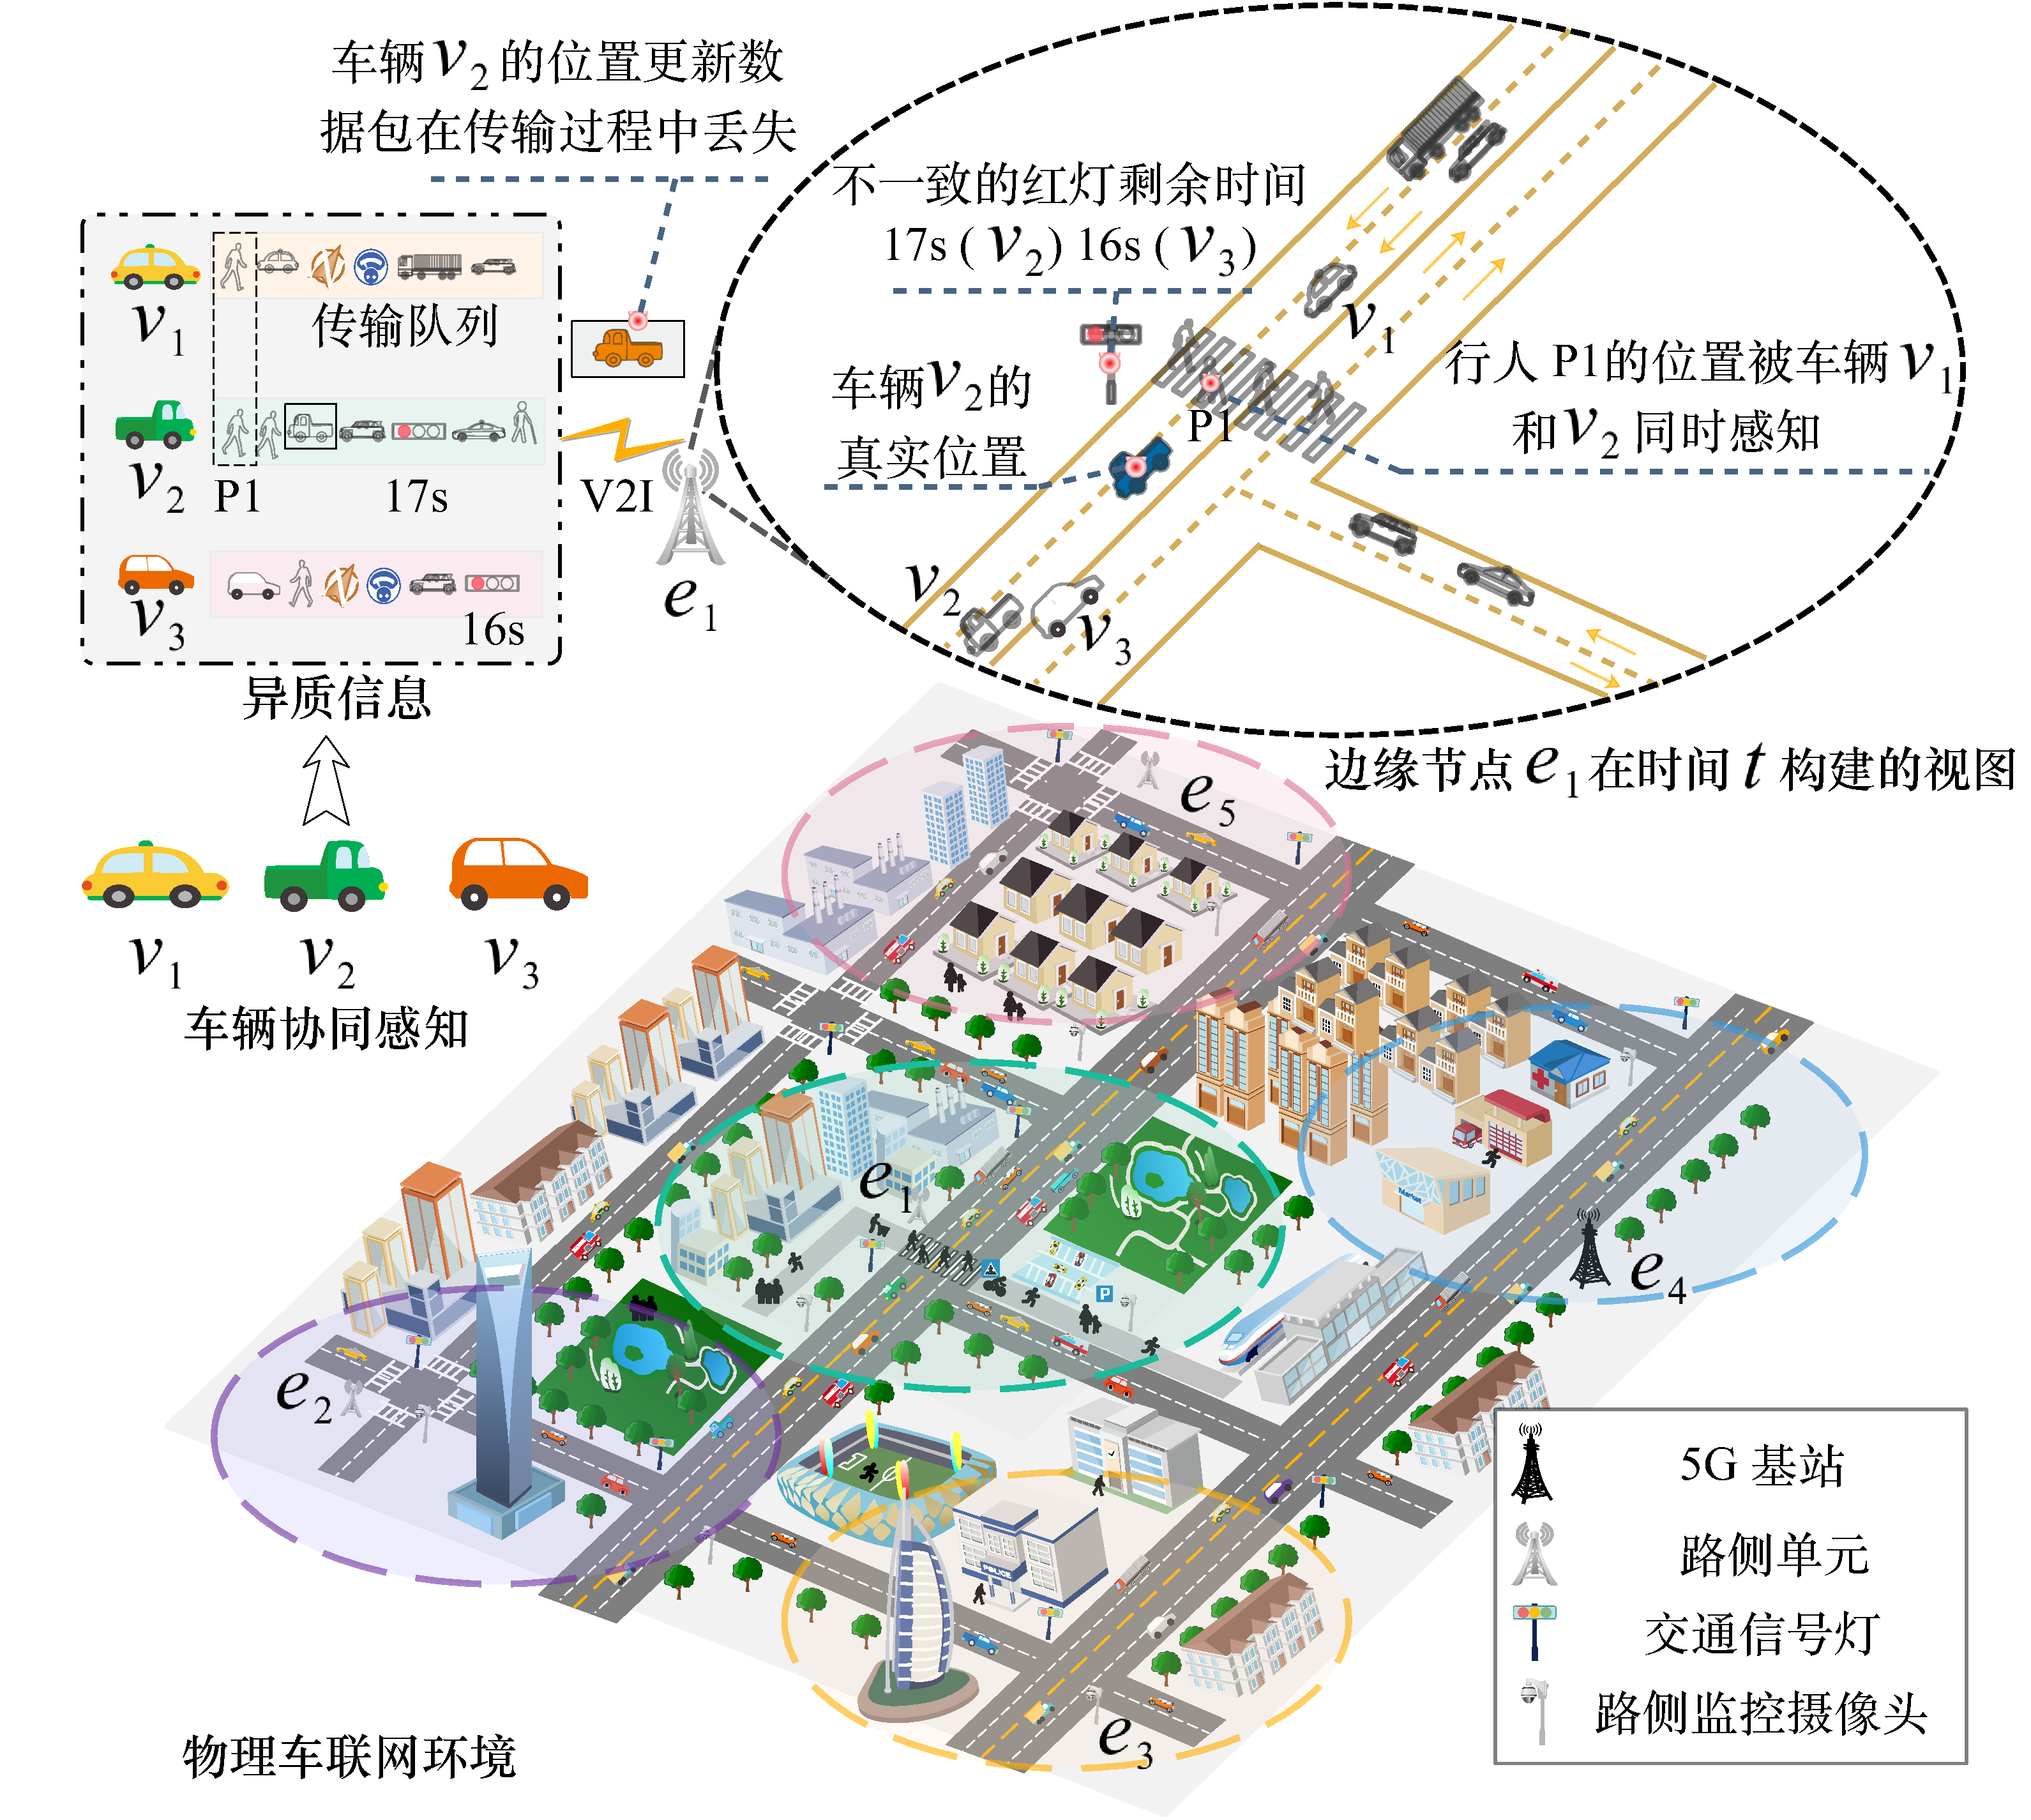
\includegraphics[width=0.7\columnwidth]{Fig2-2a-architerture.pdf}}
     \subfloat[][]{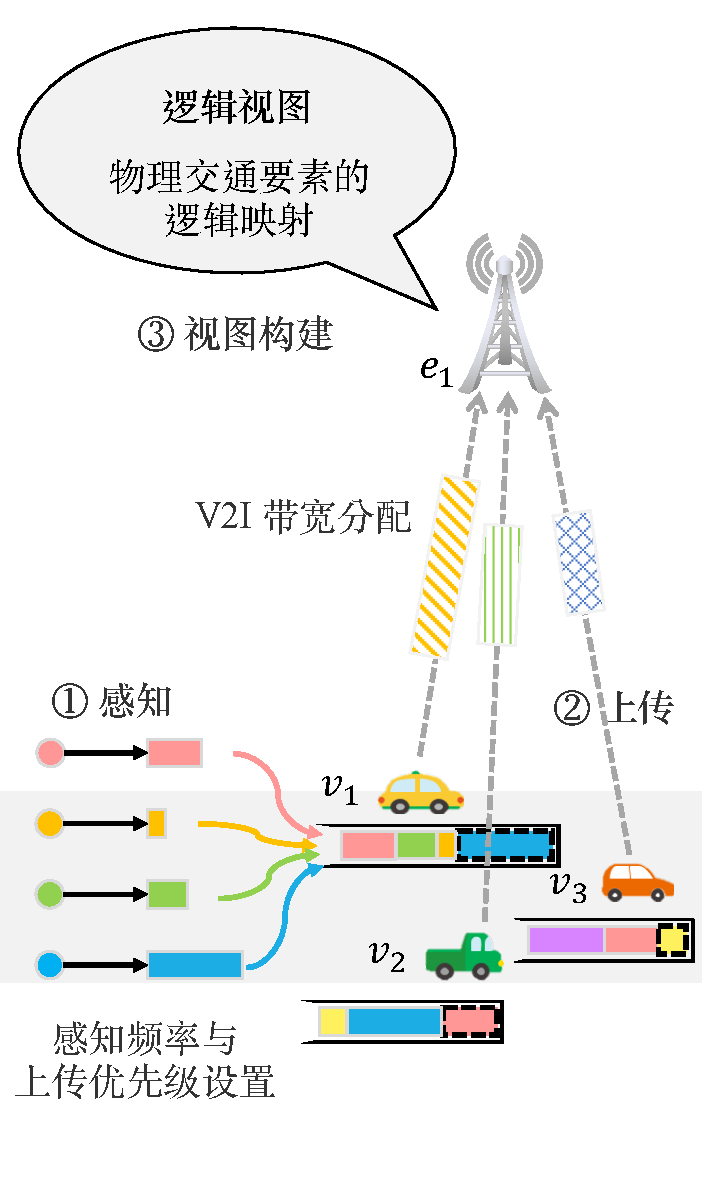
\includegraphics[width=0.3\columnwidth]{Fig2-2b-procedures.pdf}}
     \bicaption[系统场景]{系统场景。(a) 车载信息物理融合系统中分布式感知与异质信息融合 (b) 系统工作流程}[Scenario]{Scenario. (a) Distributed sensing and heterogeneous information fusion in VCPS (b) System workflow}
     \label{fig 2-2}
\end{figure}

本系统的工作流程如图\ref{fig 2-2}(b)所示,边缘节点$e_1$的逻辑视图构建包括以下三个步骤:步骤1(感知):每辆车根据其位置和感知能力感知到不同的信息。感知信息在每辆车上排队,以便上传到边缘节点。每辆车将决定这些信息的感知频率和上传优先级。由于异质信息是由车辆以不同的感知频率感知的,因此不同信息的到达时刻可能不同。同时,提高感知频率可以提高信息的新鲜度,但也会增加排队延迟。为了确定不同信息的上传优先级,必须综合考虑信息的数据量大小、V2I通信的连接性和视图需求。步骤2(上传):边缘节点将V2I带宽(即不同范围的非重叠频谱)分配给有上传任务的车辆,以便这些车辆能够同时上传他们的传感信息而不受干扰。由于边缘节点的带宽资源有限且车辆信道条件多变,分配的V2I带宽可能不足以支持及时上传数据。因此,在车辆准备上传急需的时效信息情况下,将更大的带宽分配给这些车辆,而不是分配给在更差的信道条件下的车辆(如离开V2I覆盖范围)。因此,可以通过对车辆和边缘节点之间的信噪比(Signal-to-Noise Ratio, SNR)建模来考虑了不同车辆的信道条件。同时,V2I传输速率由两个节点之间的距离和分配的带宽决定。步骤3(视图构建):边缘节点根据具体的ITS应用要求,将收到的物理信息映射到相应的逻辑元素上,从而构建逻辑视图。

此外,本章提供了一个例子来更好地说明上述观点。如图\ref{fig 2-2}(a)所示,在时间 $t$,边缘节点$e_1$构建了一个逻辑视图,并根据车辆$v_1$、$v_2$和$v_3$感知和上传的信息,在交叉路口启用了速度建议应用。一般而言,速度建议应用的目标是向正在接近交叉口的车辆提供最佳速度建议,使车辆可以顺利通过,从而达到最大化整体交通效率。假设车辆$v_2$和$v_3$都能感知交通灯信息,但感知的红灯剩余时间数值不一致,进一步导致信息不一致。同时,同一物理要素的状态可能会被多辆车同时感知到。在这种情况下,该消息只需要由其中一辆车在一定时间内上传以节省V2I带宽。只要物理要素在边缘节点以相同的质量水平建模,其就可以被应用于不同的应用,而不需要由不同的车辆重复上传。此外,数据包丢失可能导致物理车联网环境和视图之间的差距。例如,假设车辆$v_2$的位置更新数据包丢失,这会导致其真实位置与时间$t$视图上的位置之间存在明显的不一致。因此,定量评估边缘节点构建的视图的质量,并为协作感知和信息融合设计有效的调度机制,以最大限度地提高VCPS的整体质量是至关重要且具有挑战性的。

\section{车载信息物理融合质量指标设计}\label{section 2-4}

\subsection{基本符号}

系统的离散时间片集合用$\mathbf{T}=\{1, \ldots, t, \ldots, T\}$表示。
异质信息的集合用$\mathbf{D}=\{1, \ldots, d, \ldots, D\}$表示,其中信息$d$可以用一个双元组$d=\left(\operatorname{type}_d, \left|d\right| \right)$表示,其中$\operatorname{type}_d$为类型,$\left|d\right|$为数据量。
车辆的集合用$\mathbf{V}=\{1, \ldots, v, \ldots, V\}$表示,其中车辆$v$的特征用一个三元组$v=\left (l_v^t, \mathbf{D}_v, \pi_v \right )$表示,其中$l_v^t$是车辆$v$在时间$t$的位置;$\mathbf{D}_v$是车辆$v$可以感知的信息集合,$\pi_v$是车辆$v$的传输功率。
边缘节点的集合用$\mathbf{E}=\{1, \ldots, e, \ldots, E\}$表示,其中边缘节点$e$的特征用一个三元组$e=\left (l_e, g_e, b_e \right)$表示,其中$l_e$是位置,$g_e$是通信范围,$b_e$是带宽。
在时间$t$,车辆$v$与边缘节点$e$的距离表示为$\operatorname{dis}_{v,e}^t \triangleq \operatorname{distance} \left (l_v^t, l_e \right )$,其中$\operatorname{distance}\left(\cdot,\cdot\right)$是欧氏距离。

车辆$v$在时间$t$所感知的信息集合用$\mathbf{D}_v^t\subseteq \mathbf{D}_v$表示。
对于车辆在时间$t$感知到的信息类型,需要各不相同,即对于$\mathbf{D}_v^t$中的任意信息$d$,信息类型都是不同的,$\operatorname{type}_{d^*} \neq \operatorname{type}_{d}, \forall d^* \in \mathbf{D}_v^t \setminus \left\{ d\right \}, \forall d \in \mathbf{D}_v^t$。
车辆$v$在时间$t$对于信息$d$的感知频率用$\lambda_{d,v}^t$表示。
由于感知能力有限,车辆感知频率需满足$\lambda_{d,v}^{t} \in [\lambda_{d,v}^{\min} , \lambda_{d,v}^{\max} ], \forall d \in \mathbf{D}_v^t, \forall v \in \mathbf{V}, \forall t \in \mathbf{T}$, 其中 $\lambda_{d,v}^{\min}$ 和 $\lambda_{d,v}^{\max}$ 分别为车辆$v$对于类型为$\operatorname{type}_{d}$的信息的最低和最高感知频率。
车辆$v$中的信息$d$在时间$t$的上传优先级用$p_{d,v}^t$表示,且${p}_{d^*, v}^t \neq {p}_{d, v}^t, \forall d^* \in \mathbf{D}_v^t \setminus \left\{ d\right \}, \forall d \in \mathbf{D}_v^t, \forall v \in \mathbf{V}, \forall t \in \mathbf{T}$。
在时间$t$内处于边缘节点$e$的无线电覆盖范围内的车辆集合表示为$\mathbf{V}_e^t=\left \{v \vert \operatorname{dis}_{v,e}^t \leq g_e, \forall v \in \mathbf{V} \right \}, \mathbf{V}_e^t \subseteq \mathbf{V}, \forall e \in \mathbf{E}$。
边缘节点$e$在时间$t$为车辆$v$分配的V2I带宽用$b_{v, e}^t$表示,且$b_{v, e}^t \in \left [0,b_e \right], \forall v \in \mathbf{V}_e^{t}, \forall e \in \mathbf{E}, \forall t \in \mathbf{T}$。
边缘节点$e$分配的V2I带宽总和不能超过其带宽容量$b_e$,即${\sum_{\forall v \in \mathbf{V}_e^{t}}b_{v, e}^t} \leq b_e, \forall e \in \mathbf{E}, \forall t \in \mathbf{T}$。

\subsection{系统模型}
本系统分布式感知模型如图\ref{fig 2-3}所示。
车辆感知的信息到达间时间和排队时间通过多类M/G/1优先级队列(Multi-Class M/G/1 Priority Queue)\cite{qian2020minimizing}对车辆中的感知信息队列进行建模得到。
假定车辆$v$中具有相同类型$\operatorname{type}_d$的信息传输时间分布在每个时间片内保持稳定。
类型为$\operatorname{type}_d$的信息传输时间$\operatorname{\hat{g}}_{d, v, e}^t$遵循一类一般分布(General Distribution),其均值为$\alpha_{d, v}^t$,二阶矩和三阶矩分别为$\beta_{d, v}^t$和$\gamma_{d, v}^t$,那么该分布集合可以表示为:
\begin{align}
	\mathbb{P}=\left\{\hat{\mathrm{g}}_{d, v, e}^t:\right. & \mathbb{E}\left[\hat{\mathrm{g}}_{d, v, e}^t\right]=\alpha_{d, v}^t, \notag \\
	& \mathbb{E}\left[\hat{\mathrm{g}}_{d, v, e}^t-\alpha_{d, v}^t\right]^2=\beta_{d, v}^t \notag \\
	& \mathbb{E}\left[\operatorname{\hat{g}}_{d, v, e}^t-\alpha_{d, v}^t\right]^{3}=\left.\gamma_{d, v}^t \right\}
\end{align}
因此,上传负载 $\rho_{v}^{t}$ 可表示为:
\begin{equation}
    \rho_{v}^{t}=\sum_{\forall d \subseteq \mathbf{D}_v^t} \lambda_{d,v}^{t}  \alpha_{d, v}^t
\end{equation}

\begin{figure}[h]
\centering
  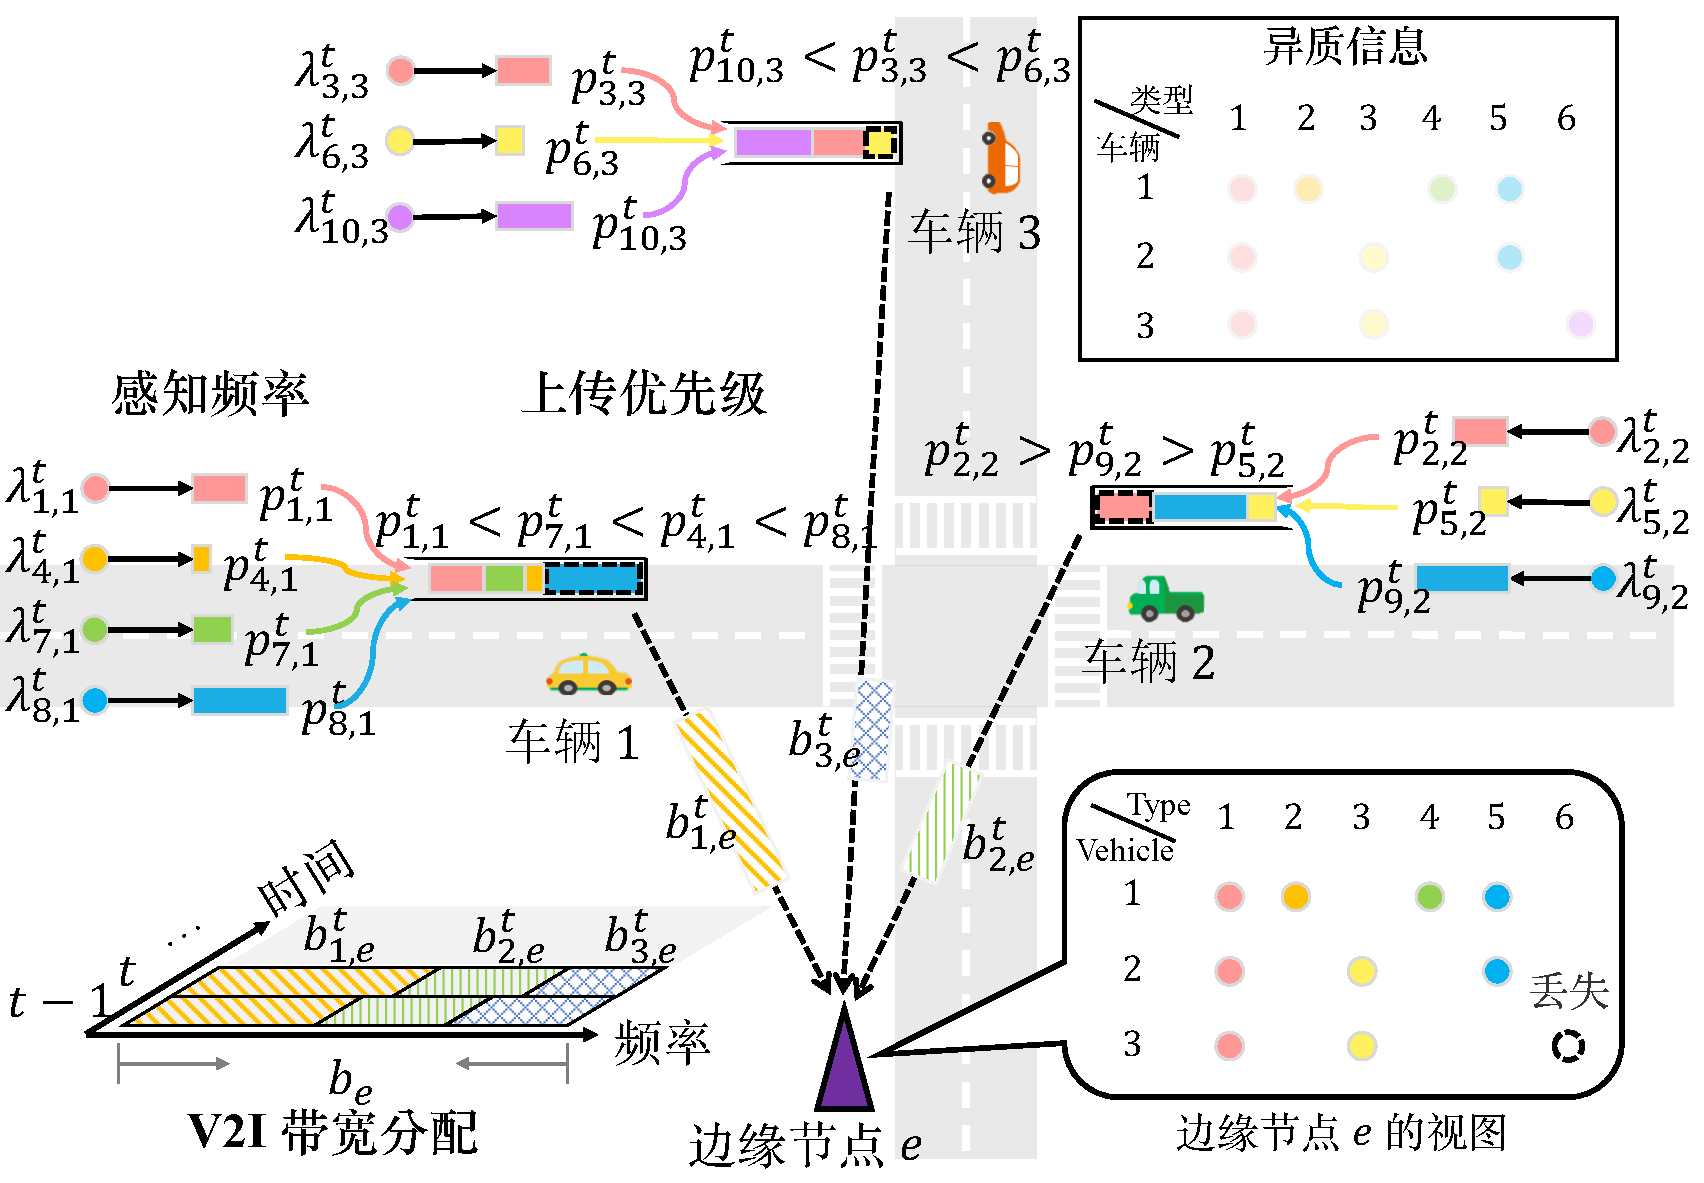
\includegraphics[width=0.8\columnwidth]{Fig2-3-cooperative-sensing.pdf}
  \bicaption{分布式感知模型}{Distributed sensing model}
  \label{fig 2-3}
\end{figure}

为了确保队列具有稳定状态,需要满足 $\rho_{v}^{t} < 1$。
到达间隔时间$\operatorname{a}_{d, v}^t$是指车辆$v$中两个相邻的具有相同类型$\operatorname{type}_d$的信息到达时间差,其计算公式为:
\begin{equation}
    \operatorname{a}_{d, v}^t=\frac{1}{\lambda_{d, v}^{t}}
\end{equation}
在时间$t$内,车辆$v$中具有比信息$d$更高上传优先级的信息集合可表示为:
\begin{equation}
\mathbf{D}_{d, v}^t=\left\{d^* \mid p_{d^*, v}^t>p_{d, v}^t, \forall d^* \in \mathbf{D}_v^t\right\} 
\end{equation}
其中$p_{d^*, v}$是信息$d^* \in \mathbf{D}_v^t$的上传优先级。
  因此,信息$d$前面的上传负载(车辆$v$在时间$t$内要在$d$前面上传的数据量)表示为:
\begin{equation}
\rho_{d, v}^t=\sum_{\forall d^* \in \mathbf{D}_{d, v}^t} \lambda_{d^*, v}^t \alpha_{d^*, v}^t
\end{equation}
其中$\lambda_{d^*, v}^t$和$\alpha_{d^*, v}^t$分别是时间$t$内车辆$v$中信息$d^*$的感知频率和平均传输时间。
车辆$v$中类型为$\operatorname{type}_d$的信息的排队时间用$\operatorname{q}_{d, v}^t$表示。
根据Pollaczek$-$Khintchine公式\cite{takine2001queue},平均排队时间$\operatorname{\bar{q}}_{d, v}^t$计算如下:
\begin{equation}
    \operatorname{\bar{q}}_{d, v}^t= \frac{1} {1 - \rho_{d, v}^{t}} 
        \left[ \alpha_{d, v}^t + \frac{ \lambda_{d, v}^{t} \beta_{d, v}^t + \sum\limits_{\forall d^* \in \mathbf{D}_{d, v}^t} \lambda_{d^*,s}^t \beta_{d^*, v}^t }{2\left(1-\rho_{d, v}^{t} - \lambda_{d, v}^{t}  \alpha_{d, v}^t\right)}\right] 
        - \alpha_{d, v}^t
\label{equ 2-6}
\end{equation}
进一步,多类M/G/1优先队列中排队时延的上界分析见附录\ref{appendix e}。

本章根据香农理论对通过V2I通信的数据上传进行建模。
在时间$t$,车辆$v$和边缘节点$e$的V2I通信的信噪比用$\operatorname{SNR}_{v, e}^{t}$表示,其计算方法如公式\ref{equ 2-7}\cite{sadek2009distributed}所示。
\begin{equation}
    \label{equ 2-7}
    \operatorname{SNR}_{v, e}^{t}=\frac{1}{N_{0}}  \left|h_{v, e}\right|^{2} \zeta  {\operatorname{dis}_{v, e}^{t}}^{-\varphi} {\pi}_v
\end{equation}
其中$N_{0}$为加性白高斯噪声(Additive White Gaussian Noise, AWGN);$h_{s, e}$为信道衰减增益;$\zeta$为取决于天线设计的常数;$\varphi$为路径损耗指数。
车辆$v$和边缘节点$e$之间在时间$t$的V2I传输率用$\operatorname{z}_{v, e}^t$表示,其计算如下: 
\begin{equation}
    \operatorname{z}_{v, e}^t=b_{v, e}^{t} \log _{2}\left(1+\mathrm{SNR}_{v, e}^{t}\right)
    \label{equ 2-8}
\end{equation}
其中$b_{v, e}^{t}$是分配给车辆$v$在时间$t$的带宽。
值得注意的是,给定车辆$v$的传输功率$\pi_s$,车辆$v$和边缘节点$e$之间在时间$t$的V2I通信的信噪比可以通过公式\ref{equ 2-7}得到,进一步可由公式\ref{equ 2-8}得到传输速率。
因此,信息$d$从车辆$v$到边缘节点$e$的传输时间用$\mathrm{w}_{d, v, e}^t$表示,其计算公式为:
\begin{equation}
	\mathrm{w}_{d, v, e}^t=\frac{\left|d\right|}{\operatorname{z}_{v, e}^t}
\end{equation}
成功传输需要在数据包传输过程中,接收到的信噪比高于某个阈值,其被称为 SNR Wall \cite{tandra2008snr},该阈值通过以下方式获得:
\begin{equation}
\mathrm{SNR}_{\text {wall }}=\frac{\sigma^{2}-1}{\sigma}
\end{equation}
其中$\sigma=10^{\nu / 10}$,$\nu$是以dB衡量的参数,量化了噪声不确定性的大小。
\begin{equation}
	\left(\nu^2 - 1\right) {N_0}={\pi_v} \nu
\end{equation}
因此,表示信息$d$是否从车辆$v$成功传输到边缘节点$e$的成功传输指示器表示为:
\begin{numcases}{\operatorname{c}_{d, v, e}^t=}
1, \forall {t^{*}} \in\left[t + \operatorname{\bar{q}}_{d, v}^t, t + \operatorname{\bar{q}}_{d, v}^t + \operatorname{w}_{d, v, e}^t\right], \operatorname{SNR}_{v, e}^{t^{*}}>\mathrm{SNR}_{\text {wall }} \notag \\
0, \exists {t^{*}} \in\left[t + \operatorname{\bar{q}}_{d, v}^t, t + \operatorname{\bar{q}}_{d, v}^t + \operatorname{w}_{d, v, e}^t\right], \operatorname{SNR}_{v, e}^{t^{*}} \leq \mathrm{SNR}_{\text {wall }}
\end{numcases}
由车辆$v$传输并由边缘节点$e$接收的信息集合表示为 $\mathbf{D}_{v, e}^t = \{ d \mid \operatorname{c}_{d, v, e}^t = 1, \forall d \in \mathbf{D}_v \}, \mathbf{D}_{v, e}^t \subseteq \mathbf{D}_v^t, \forall v \in \mathbf{V}, \forall e \in \mathbf{E}$。

\subsection{Age of View}
系统中的视图集合用$\mathbf{I}$表示,视图$i \in \mathbf{I}$所需的信息集用$\mathbf{D}_{i}$表示,它是特定ITS应用所需的物理交通元素的映射,它表示为:
\begin{equation}
	\mathbf{D}_{i} = \{d \mid y_{d, i} = 1, \forall d \in \mathbf{D} \}
\end{equation}
视图$i$所需元素的数量用$|\mathbf{D}_{i}|$表示。
边缘节点$e$在时间$t$所需的视图集合用$\mathbf{I}_e^t \subseteq \mathbf{I}$表示。
因此,边缘节点$e$收到的并被视图$i$需要的信息集用下式表示:
\begin{equation}
    \mathbf{D}_{i, e}=\bigcup_{\forall i \in \mathbf{I}}\left(\mathbf{D}_i \cap \mathbf{D}_{v, e}^t\right), \forall v \in \mathbf{V}_e^t, \forall e \in \mathbf{E}
\end{equation}
且$| \mathbf{D}_{i, e} |$是边缘节点$e$收到并被视图$i$需要的信息数量。
接下来,定义异质信息融合的三个特征,包括视图的时效性、完整性和一致性。

首先,异质信息是随时间变化的,信息的新鲜度对于视图质量至关重要。
因此,车辆$v$中的信息$d$的时效性定义如下:
\begin{definition}
	车辆$v$的信息$d$的时效性 $\xi_{d,v} \in (0, +\infty)$被定义为信息$d$的间隔到达时间、排队时间和传输时间之和。
	\begin{equation}
    	\xi_{d, v} = \operatorname{a}_{d, v}^t + \operatorname{q}_{d, v}^t + \operatorname{w}_{d, v, e}^t, \forall d \in \mathbf{D}_v^t, \forall v \in \mathbf{V}
	\end{equation}
\end{definition}
\noindent 其中 $\operatorname{a}_{d, v}^t$、$\operatorname{q}_{d, v}^t$ 和 $\operatorname{w}_{d, v, e}^t$ 分别为信息$d$的间隔到达时间、排队时间和传输时间。
进一步,视图的时效性定义如下:
\begin{definition}
视图$i$的时效性 $\Xi_{i} \in (0,+\infty)$被定义为信息时效性总和。
	\begin{equation}
    	\Xi_{i} = \sum_{\forall v \in \mathbf{V}} \sum_{\forall d \in \mathbf{D}_{i, e} \cap \mathbf{D}_v^t } \xi_{d, v}, \forall i \in \mathbf{I}_e^t, \forall e \in \mathbf{E}
	\end{equation}
\end{definition}

其次,车联网具有包括车辆高移动性、网络资源有限性和无线通信不可靠的固有特性。
由于车辆和边缘节点之间的无线传输连接断开,或者传输过程中数据包的丢失,视图可能是不完整的。
因此,视图的完整性定义如下:
\begin{definition}
	视图$i$的完整性$\Phi_{i} \in [0,1]$被定义为边缘节点$e$实际收到的信息数量与所需总量之比。
	\begin{equation}
	\Phi_{i}= {| \mathbf{D}_{i, e} |} \big/ {|D_{i} |}, \forall i \in \mathbf{I}_e^t, \forall e \in \mathbf{E}
	\end{equation}
\end{definition}
\noindent 其中$|\mathbf{D}_{i, e}|$是边缘节点$e$收到并被视图$i$需要的信息数量,$|\mathbf{D}_{i}|$是视图$i$需要的信息总数量。

再次,由于不同类型的信息有各自的感知频率和上传优先级,在构建视图时,需要使不同类型信息的版本尽可能接近。
因此,视图的一致性定义如下: 
\begin{definition}
视图$i$的一致性$\Psi_{i} \in (0,+\infty)$被定义为信息接收时间与视图所需信息的平均接收时间之差的二次方和。
\begin{equation}
\Psi_{i}=\sum_{\forall v \in \mathbf{V}} \sum_{\forall d \in \mathbf{D}_{i, e} \cap \mathbf{D}_v^t} \left|\operatorname{q}_{d, v}^t + \operatorname{w}_{d, v, e}^t - \psi_{i} \right|^{2}, \forall i \in \mathbf{I}_e^t, \forall e \in \mathbf{E}
\end{equation}
\end{definition}
\noindent 其中 $\psi_{i}$ 是视图$i$所需信息的平均接收时间,其可由下式得到:
\begin{equation}
	\psi_{i} = \frac{1}{|D_{i, e}|} {\sum_{\forall v \in \mathbf{V}}\sum_{\forall d \in D_{i, e} \cap \mathbf{D}_v^t} \left( \operatorname{q}_{d, v}^t + \operatorname{w}_{d, v, e}^t\right) }, \forall i \in\mathbf{I}_e^t, \forall e \in \mathbf{E}
\end{equation}

最后,本章给出了Age of View的正式定义,其综合了视图的时效性、完整性和一致性。
\begin{definition}
Age of View $\operatorname{AoV}_{i} \in (0, 1)$ 被定义为视图$i$的归一化时效性、完整性和一致性的加权平均值。
	\begin{equation}
	    \operatorname{AoV}_{i} = w_1  \hat{\Xi}_{i} + w_2  \hat{\Phi}_{i}+  w_3 \hat{\Psi}_{i}, \forall i \in \mathbf{I}_e^t, \forall e \in \mathbf{E}
\end{equation}
\end{definition}
\noindent 其中,$\hat{\Xi}_{i} \in (0, 1)$、$\hat{\Phi}_{i} \in (0, 1)$和$\hat{\Psi}_{i} \in (0, 1)$分别表示视图$i$的归一化时效性、归一化完整性和归一化一致性。
$\operatorname{AoV}_{i}$的值越低,说明构建的视图质量越高。
需要注意的是,由于视图的时效性、完整性和一致性的维度不同,为了形成AoV的统一表示,将它们归一化到$(0,1)$范围内,具体如下:
\begin{numcases}{}
\hat{\Xi}_{i} = {\Xi}_{i} \big/ \left( \delta_\xi | \mathbf{D}_{v, e} |   T \right) \notag \\ 
\hat{\Phi}_{i} = 1 - {\Phi}_{i}  \notag \\
\hat{\Psi}_{i} = {\Psi}_{i} \big/ \left( \delta_\psi  \max\limits_{\substack{\forall d \in \mathbf{D}_v \cap \mathbf{D}_v^t \\ \forall v \in \mathbf{V}}}{\left\{ \left|\operatorname{q}_{d, v}^t + \operatorname{g}_{d, v, e}^t - \psi_{i} \right|^{2}\right\}}   \right)
\end{numcases}
\noindent 其中$\delta_{\xi} \in(0,1)$和$\delta_\psi \in(0,1)$分别是时效性和一致性的数据比例系数,通过缩减时效性和一致性的理论最大值避免归一化结果将大部分数值集中在一个小范围内。
$\hat{\Xi}_{i}$、$\hat{\Phi}_{i}$和$\hat{\Psi}_{i}$的加权系数分别用$w_1$、$w_2$和$w_3$表示,且$w_1+w_2+w_3=1$。
加权系数可以根据ITS应用的不同要求进行相应的调整。
例如,对于道路交叉口的速度咨询应用,车辆需要从边缘节点接收实时速度的指令,以便安全顺利地通过交叉口。
在这种情况下,时效性因素(例如,实时交通灯状态)与完整性因素(例如,行人在视图中被建模)相比,在视图建模中更为重要。

\subsection{问题定义}
鉴于上述指标AoV是单独评估视图的质量,本章进一步在系统层面上定义VCPS的质量如下:
\begin{definition}
VCPS的质量$\Upsilon \in (0,1)$被定义为在调度期$\mathbf{T}$中边缘节点的每个视图$i$的AoV的补集平均值。
\begin{equation}
\Upsilon=\frac{\sum_{\forall t \in \mathbf{T}} \sum_{\forall e \in \mathbf{E}} \sum_{\forall i \in \mathbf{I}_e^t} \left(1 - \operatorname{AoV}_{i}\right)}{\sum_{\forall t \in \mathbf{T}} \sum_{\forall e \in \mathbf{E}} |\mathbf{I}_e^t| }
\end{equation}
\end{definition}

给定一个确定性的解决方案$(\bf\Lambda, \mathbf{P}, \mathbf{B} )$,其中$\bf\Lambda$表示确定的感知频率,$\mathbf{P}$表示确定的上传优先级,$\mathbf{B}$表示确定的V2I带宽分配,它们分别表示为:
\begin{numcases}{}
{\bf\Lambda} = \left\{ \lambda_{d, v}^{t} \vert \forall d \in \mathbf{D}_v^t  , \forall v \in \mathbf{V}, \forall t \in \mathbf{T} \right\} \notag \\ 
\mathbf{P} = \left \{ p_{d, v}^{t} \vert \forall d \in \mathbf{D}_v^t  , \forall v \in \mathbf{V}, \forall t \in \mathbf{T}\right \} \notag \\
\mathbf{B} = \left \{ b_{v, e}^t \vert \forall v \in \mathbf{V}_e^t, \forall e \in \mathbf{E}, \forall t \in \mathbf{T}\right \}
\end{numcases}
\noindent 其中,$\lambda_{d,v}^{t}$ 表示车辆$v$在时间$t$对信息$d$的感知频率,$p_{d, v}^{t}$ 表示车辆$v$在时间$t$对信息$d$的上传优先级,$b_{v, e}^t$ 表示边缘节点$e$在时间$t$为车辆$v$分配的V2I 带宽。

本章旨在通过车辆间分布式感知与边缘节点的异质信息融合以构建边缘视图并进一步实现高质量车载信息物理融合。
本章的目标问题是通过确定所有车辆上不同信息感知频率、上传优先级,以及边缘节点对于通信覆盖范围内所有车辆进行V2I带宽分配,以最大限度地提高VCPS的质量。
因此,最大化VCPS质量问题形式化定义如下:
\begin{align}
	&\max_{\bf\Lambda, \mathbf{P}, \mathbf{B}} \Upsilon \notag \\
	\text { s.t. }
    \mathcal{C}2.1: & \lambda_{d,v}^{t} \in \left [\lambda_{d,v}^{\min} , \lambda_{d,v}^{\max} \right ], \forall d \in \mathbf{D}_v^t , \forall v \in \mathbf{V}, \forall t \in \mathbf{T} \notag \\
     \mathcal{C}2.2: &{p}_{d^*, v}^t \neq {p}_{d, v}^t, \forall d^* \in \mathbf{D}_v^t \setminus \left\{ d\right \}, \forall d \in \mathbf{D}_v^t, \forall v \in \mathbf{V}, \forall t \in \mathbf{T} \notag \\
    \mathcal{C}2.3: & b_{v, e}^t \in \left[ 0 , b_e \right ], \forall v \in \mathbf{V}_e^t, \forall e \in \mathbf{E}, \forall t \in \mathbf{T} \notag \\
    \mathcal{C}2.4: & \sum_{\forall d \subseteq \mathbf{D}_v^t} \lambda_{d,v}^{t}  \alpha_{d, v}^t < 1,\ \forall v \in \mathbf{V}, \forall t \in \mathbf{T}  \notag \\
    \mathcal{C}2.5: & {\sum_{\forall v \in \mathbf{V}_e^{t}}b_{v, e}^t} \leq b_e, \forall e \in \mathbf{E}, \forall t \in \mathbf{T}
\end{align}
约束条件$\mathcal{C}2.1$要求车辆$v$中的信息$d$在时间$t$的感知频率应满足其感知能力的要求。
$\mathcal{C}2.2$ 保证时间$t$内车辆$v$中信息$d$的上传优先级。
$\mathcal{C}2.3$ 规定边缘节点$e$在时间$t$为车辆$v$分配的V2I带宽不能超过其带宽容量$b_e$。
$\mathcal{C}2.4$保证在调度周期$\mathbf{T}$内队列稳定状态。
$\mathcal{C}2.5$要求边缘节点$e$分配的V2I带宽之和不能超过其容量$b_e$。

\section{基于差分奖励的多智能体强化学习算法设计}\label{section 2-5}

\subsection{算法模型}
本章将详细介绍所提基于差分奖励的多智能体深度强化学习算法,其模型如图\ref{fig 2-4}所示,由$V$辆车、边缘节点$e$、VCPS环境和经验回放缓存组成。
首先,车辆$v$决定其动作$\boldsymbol{a}_{v}^{t}$,包括确定感知频率和上传优先级。
特别地,车辆$v$动作由行动者网络生成,其输入是对系统状态的局部观测$\boldsymbol{o}_{v}^{t}$。
车辆$v$的评论家网络评估由相应行动者网络产生的动作。
其次,边缘节点$e$根据车辆预测轨迹和视图需求决定其动作$\boldsymbol{a}_{e}^{t}$,即为通信覆盖范围内的车辆分配V2I带宽。
再次,环境根据动作$\{ \boldsymbol{a}_{1}^{t}, \ldots, \boldsymbol{a}_{v}^{t}, \ldots, \boldsymbol{a}_{V}^{t}, \boldsymbol{a}_{e}^{t}\}$ 获得系统奖励,即边缘节点$e$在时间$t$实现的VCPS质量。
并采用基于差分奖励\cite{foerster2018counterfactual}的信用分配,将系统奖励分为差分奖励$\{r_1^t, \ldots, r_{V}^t\}$,其中$r_v^t$被用来评估车辆$v$对视图构建的贡献。
最后,相关的交互经验包括当前系统状态、车辆动作、差分奖励和下一时刻系统状态,都存储在经验回放缓存中,并用来训练车辆的行动者和评论家网络。
算法模型的主要组成部分设计如下:

1) \textbf{系统状态}: 边缘节点定期广播其视图需求和缓存信息。在时间$t$内,车辆$v$的系统状态的本地观测被表示为:
	\begin{equation}
		\boldsymbol{o}_{v}^{t}=\left\{\mathbf{D}_{v}^{t}, \mathbf{D}_{e}^{t}, \mathbf{I}_e^t\right\}
	\end{equation} 
	\noindent 其中$\mathbf{D}_{v}^{t}$表示车辆$v$在时间$t$感知的信息集合;
	$\mathbf{D}_{e}^{t}$ 表示在时间$t$边缘节点$e$中的缓存信息集合,
	以及$\mathbf{I}_e^t$表示边缘节点$e$在时间$t$的边缘节点所需的视图集合。
	那么,时间$t$的系统状态可表示为:
	\begin{equation}
		\boldsymbol{o}^{t}=\left\{\mathbf{D}_{1}^{t}, \ldots, \mathbf{D}_{v}^{t}, \ldots, \mathbf{D}_{V}^{t}, \mathbf{D}_{e}^{t}, \mathbf{I}_{e}^{t}\right\}
	\end{equation}
	
\begin{figure}[t]
\centering
  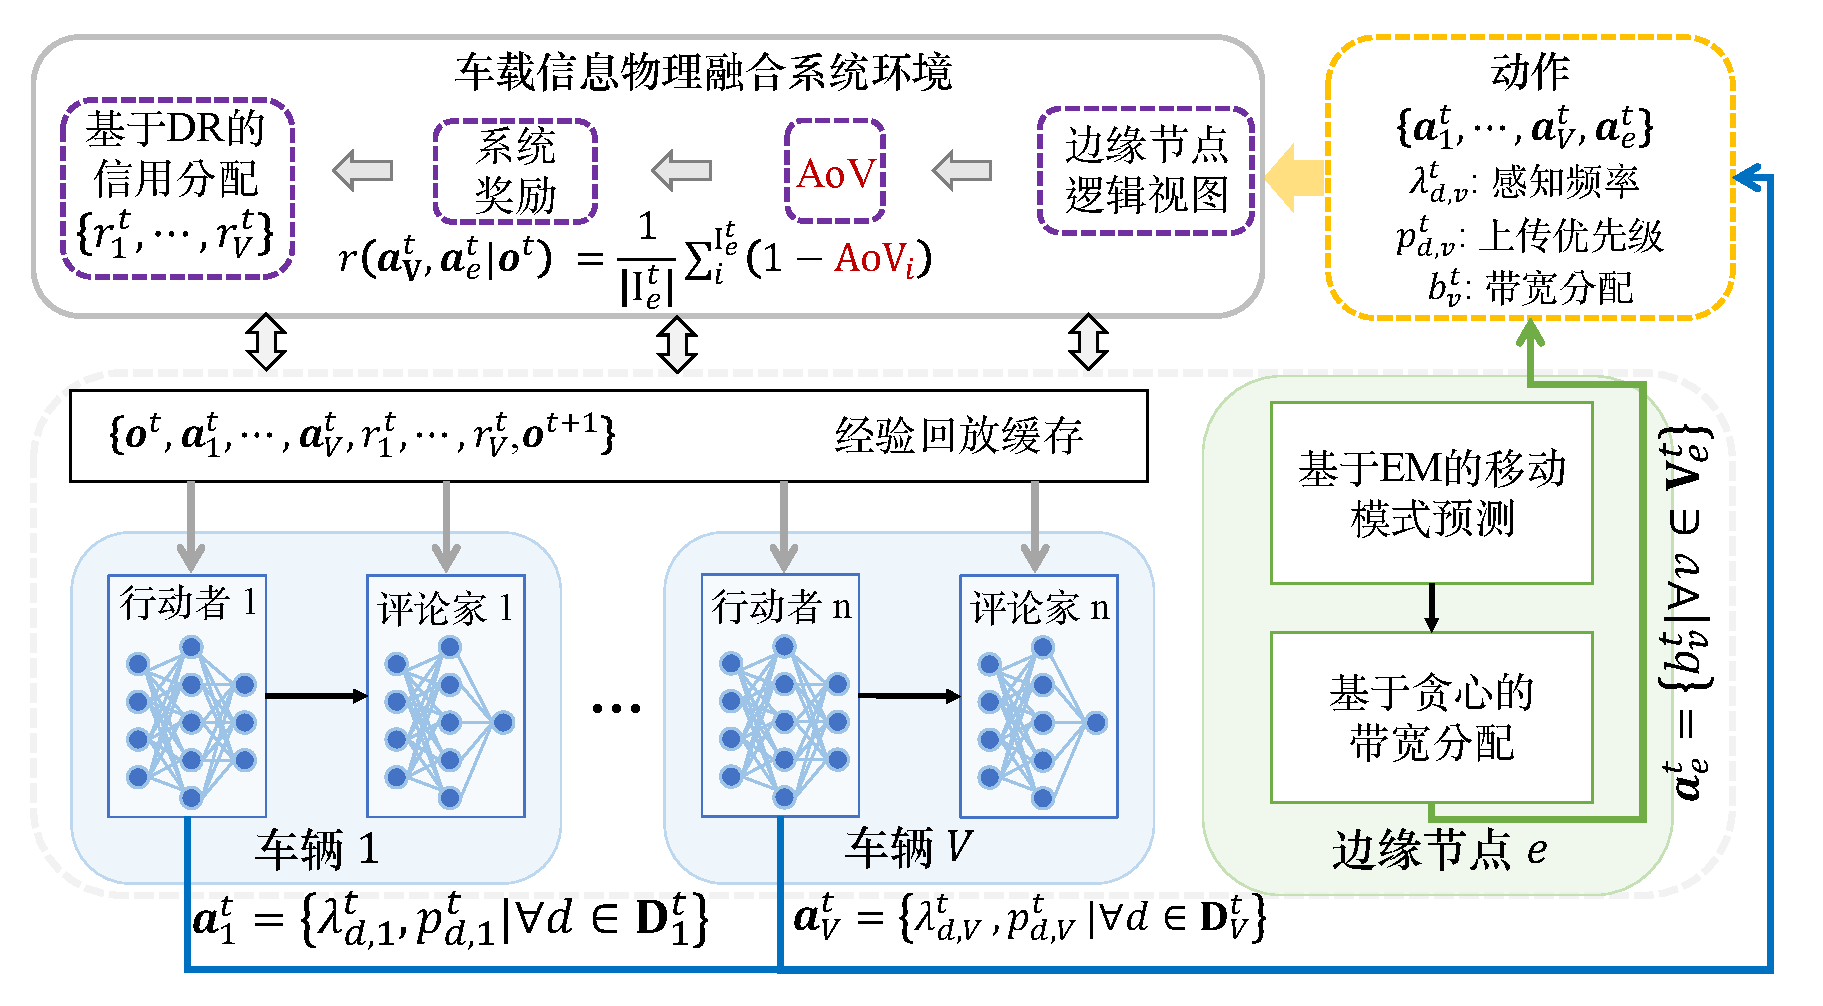
\includegraphics[width=1\columnwidth]{Fig2-4-solution-model.pdf}
  \bicaption{基于差分奖励的多智能体深度强化学习模型}{Multi-agent difference-reward-based deep reinforcement learning model}
  \label{fig 2-4}
\end{figure}

2) \textbf{动作空间}: 车辆$v$的动作空间由时间$t$的感知频率和传感信息的上传优先级组成,它被表示为:
	\begin{equation}
		\boldsymbol{a}_{v}^{t}=\{ \lambda_{d, v}^{t}, p_{d, v}^{t} \mid \forall d \in \mathbf{D}_{v}^t\}
	\end{equation}
	\noindent 其中$\lambda_{d, v}^{t}$和$p_{d, v}^{t}$分别是时间$t$内车辆$v$中信息$d$的感知频率和上传优先级。
	车辆动作的集合用$\boldsymbol{a}_{\mathbf{V}}^{t} = \left\{\boldsymbol{a}_{v}^{t}\mid \forall v \in \mathbf{V}\right\}$表示。
	边缘节点的动作是对车辆进行V2I带宽分配,其表示为:
	\begin{equation}
		\boldsymbol{a}_{e}^{t}=\{b_{v, e}^{t} \mid \forall v \in \mathbf{V}_{e}^{t}\}
	\end{equation}
	其中$b_{v, e}^t$是边缘节点$e$在时间$t$为车辆$v$分配的V2I带宽。
	
3) \textbf{系统奖励}: 在系统状态$\boldsymbol{o}^{t}$下,通过车辆动作$\boldsymbol{a}_{\mathbf{V}}^{t}$和边缘节点动作$\boldsymbol{a}_{e}^{t}$的系统奖励被定义为$t$时边缘节点$e$实现的VCPS质量,其计算公式为:
	\begin{equation}
		r\left(\boldsymbol{a}_{\mathbf{V}}^{t},\boldsymbol{a}_{e}^{t} \mid \boldsymbol{o}^{t}\right)=\frac{1}{\left|\mathbf{I}_e^t\right|} \sum_{\forall i \in \mathbf{I}_e^t}\left(1 -\operatorname{AoV}_{i} \right)
	\end{equation}
	
系统奖励展示了整个系统的综合表现,该表现来自于车辆和边缘节点的共同努力。
为了评估各车辆的贡献,需要将系统奖励分配给每个车辆作为个人奖励。
基于DR的信用分配方案是通过计算系统奖励与无该智能体动作所获奖励之间的差值来确定该智能体的个人奖励,可以更准确地评估每个智能体的行为,从而进一步提升所提出解决方案的性能。
因此,车辆$v$的差分奖励表示为:
\begin{equation}
r_{v}^{t}=r\left(\boldsymbol{a}_{\mathbf{V}}^{t},\boldsymbol{a}_{e}^{t} \mid \boldsymbol{o}^{t}\right)-r\left(\boldsymbol{a}_{\mathbf{V}-v}^{t},\boldsymbol{a}_{e}^{t} \mid \boldsymbol{o}^{t}\right)
\end{equation}
\noindent 其中 $r\left(\boldsymbol{a}_{\mathbf{V}-v}^{t},\boldsymbol{a}_{e}^{t} \mid \boldsymbol{o}^{t}\right)$是没有车辆$v$贡献的系统奖励,其可通过设置车辆$v$的空动作集得到。
车辆的差分奖励集合用$\boldsymbol{r}_{\mathbf{V}}^{t}=\{ r_{v}^{t} \mid \forall v \in \mathbf{V}\}$表示。

\subsection{工作流程}
本章节介绍基于差分奖励的多智能体强化学习算法的工作流程,其主要包括三个部分,即初始化、回放经验存储和训练,其详细步骤见算法2.1。

1) \textbf{初始化}: 首先,每辆车都作为一个智能体并由四个神经网络组成,即一个本地行动者网络、一个目标行动者网络、一个本地评论家网络和一个目标评论家网络。
车辆$v$的本地行动者和本地评价家网络的参数分别用$\theta_{v}^{\mu}$和$\theta_{v}^{Q}$来表示。
目标行动者和目标评论家网络的参数分别用$\theta_{v}^{\mu^{\prime}}$和$\theta_{v}^{Q^{\prime}}$表示。
其次,车辆的本地行动者和本地评价家网络的参数通过随机方式进行初始化。
目标行动者和目标评论家网络的参数初始化为与相应的本地网络一致。
\begin{align}
	\theta_{v}^{\mu^{\prime}} \leftarrow \theta_{v}^{\mu}, \forall v \in \mathbf{V}\\
	\theta_{v}^{Q^{\prime}} \leftarrow \theta_{v}^{Q}, \forall v \in \mathbf{V}
\end{align}
最后,初始化一个最大容量为$|\mathcal{B}|$的经验回放缓存以存储车辆与环境的交互经验。

\SetKwInOut{KwIn}{输入}
\SetKwInOut{KwOut}{输出}

\begin{algorithm}[h]\small
\renewcommand{\algorithmcfname}{算法}
		\caption{基于差分奖励的多智能体深度强化学习}
		\KwIn{学习率$\alpha$和$\beta$、折扣因子$\tau$、经验回放缓存$\mathcal{B}$、批大小$M$、轨迹预测时间$H$}
		\KwOut{信息感知频率$\lambda_{d, v}^{t}$、上传优先级$p_{d, v}^{t}$、带宽分配$b_{v, e}^{t}$}
		初始化网络参数\\
		初始化经验回放缓存$\mathcal{B}$\\
        \For{\songti{迭代次数} $= 1$ \songti{到最大迭代次数}}{
            初始化一个随机过程 $\mathcal{N}$ 以进行探索 \\
            接收初始系统状态 $\boldsymbol{o}_{1}$\\
            \For{\songti{时间片} $t = 1$ \songti{到} $T$}{
            	\For{\songti{车辆} $v=1$ \songti{到} $V$ }{
            			接收本地观测值 $\boldsymbol{o}_{v}^{t}$ \\
                    	选择一个动作 $\boldsymbol{a}_{v}^{t}=\boldsymbol{\mu}_{v}\left(\boldsymbol{o}_{v}^{t} \mid \theta_{v}^{\mu}\right)+\mathcal{N}_{t}$ \\
            		得到所需信息 $\mathbf{D}_{v,\operatorname{R}}^{t}$\\
        		通过基于EM方法利用历史相对距离来预测移动模式\\
        		预测未来的轨迹 $\operatorname{Traj}_{v}^{t}$ \\
        		计算平均距离$\operatorname{\bar{dis}}_{v, e}^{t}$
            	}
        	\For{\songti{车辆} $v=1$ \songti{到} $V$ }{
        		通过VBA策略分配带宽 $b_{v, e}^{t}$ 给车辆 $s$\\}
            	接收系统奖励 $r\left(\boldsymbol{a}_{\mathbf{V}}^{t},\boldsymbol{a}_{e}^{t} \mid \boldsymbol{o}^{t}\right)$ 和下一时刻系统状态 $\boldsymbol{o}^{t+1}$\\
            	划分系统奖励为差分奖励$\boldsymbol{r}_{\mathbf{V}}^{t}$\\
            	存储 $\left(\boldsymbol{o}^{t}, \boldsymbol{a}_{\mathbf{V}}^{t}, \boldsymbol{r}_{\mathbf{V}}^{t}, \boldsymbol{o}^{t+1}\right)$ 到经验回放缓存 $\mathcal{B}$
            }
            \For{\songti{车辆} $v=1$ \songti{到} $V$ }{
            		从经验回放缓存$\mathcal{B}$随机采样 $M$ 最小批\\
            		更新本地行动者和评论家网络参数\\
            	}
            	更新目标行动者和评论家网络参数
       	}
\label{algorithm 2-1}
\end{algorithm}

2) \textbf{回放经验存储}:
在每次迭代的开始,初始化一个随机过程$\mathcal{N}$用于增加智能体探索。
车辆$v$在时间$t$的行动是由本地行动者网络根据其对系统状态的本地观察得到的。
\begin{equation}
	\boldsymbol{a}_{v}^{t}=\boldsymbol{\mu}_{\boldsymbol{v}}\left(\boldsymbol{o}_{v}^{t} \mid \theta_{v}^{\mu}\right)+\mathcal{N}_{t}
\end{equation}
\noindent 其中,$\mathcal{N}_{t}$是一个由随机过程$\mathcal{N}$得到的探索噪音,以增加车辆动作的多样性。

边缘节点$e$根据车辆预测轨迹和视图需求,通过VBA方案分配V2I带宽。
首先,边缘节点$e$根据车辆和边缘节点之间的历史距离,使用期望最大化(Expectation-Maximization, EM)方法\cite{hofmann2001unsupervised} 预测车辆的移动模式。
然后,根据基于EM的移动性预测模式,预测车辆$v$在未来$H$时间片的轨迹,用$\operatorname{Traj}_{v}^{t} = \{ \hat{l}_{v}^{t+1}, \dots, \hat{l}_{v}^{t+h}, \dots, \hat{l}_{v}^{t+H}\}$表示,其中$\hat{l}_{v}^{t+h}$是车辆$v$在时间$t+h$的预测位置。
因此,车辆在边缘节点之间的平均距离的计算公式如下:
\begin{equation}
	\operatorname{\bar{dis}}_{v, e}^{t} = \frac{1}{H} {\sum_{\forall h \in [1, H]} \widehat{\operatorname{dis}}_{v, e}^{t+h}}
\end{equation}
其中,$\widehat{\operatorname{dis}}_{v, e}^{t+h}$ 是车辆$v$预测位置与边缘节点的距离,即$\widehat{\operatorname{dis}}_{v, e}^{t+h}=\operatorname{distance}(\hat{l}_{v}^{t+h}, l_{e})$。

那么,由车辆$v$感知到的并被视图$i$在时间$t$所需的信息集表示为:
\begin{equation}
	\mathbf{D}_{v, i}^{t} = \left\{ d \mid  d \in \mathbf{D}_{v}^t \cap  \mathbf{D}_i \right\}
\end{equation}
因此,由车辆$v$感知并被边缘节点$e$上视图在时间$t$需要的信息集合表示为:
\begin{equation}
	\mathbf{D}_{v, {\mathbf{I}_e^t}}^{t} = \{ d \mid  d \in \bigcup_{\forall v \in V_e^t} \mathbf{D}_{v, i}^{t}\}
\end{equation}
\noindent 该集合的大小记为$|\mathbf{D}_{v, {\mathbf{I}_e^t}}^{t}|$, 并可通过下式得到:
\begin{equation}
	|\mathbf{D}_{v, {\mathbf{I}_e^t}}^{t}| = \sum_{\forall d \in \mathbf{D}_{v, {\mathbf{I}_e^t}}^{t}}|d|
\end{equation}
最后,边缘节点$e$为车辆$v$分配的V2I带宽由下式计算:
\begin{equation}
	b_{v, e}^{t} =\frac{b_{e}} {\omega+\operatorname{rank}_{v}}
\end{equation}
\noindent 其中$\omega$为常数,$\operatorname{rank}_{v}$为车辆$v$按$| \mathbf{D}_{v, {\mathbf{I}_e^t}}^{t}|$的序列降序并按$\operatorname{\bar{dis}}_{v, e}^{t}$的序列升序排列的序列名次。

在确定车辆和边缘节点的联合动作后,以实现的VCPS质量作为系统奖励$r\left(\boldsymbol{a}_{\mathbf{V}}^{t},\boldsymbol{a}_{e}^{t} \mid \boldsymbol{o}^{t}\right)$,并通过基于DR的信用分配方案进一步划分为差分奖励$\boldsymbol{r}_{\mathbf{V}}^{t}$。
最后,包括当前系统状态$\boldsymbol{o}^{t}$、车辆动作$\boldsymbol{a}_{\mathbf{V}}^{t}$、差分奖励$\boldsymbol{r}_{\mathbf{V}}^{t}$和下一时刻系统状态$\boldsymbol{o}^{t+1}$在内的交互经验被存储在经验回放缓存$\mathcal{B}$。

3) \textbf{训练}: 从经验回放缓存$\mathcal{B}$中随机抽取$M$样本的小批量,用于训练车辆中的行动者和评论家网络,其中单个样本用$(\boldsymbol{o}_{v}^{m}, \boldsymbol{a}_{\mathbf{V}}^{m}, \boldsymbol{r}_{\mathbf{V}}^{m}, \boldsymbol{o}_{v}^{m+1})$表示。
本地行动者网络和本地评论家网络的参数以学习率$\alpha$和$\beta$更新
车辆$v$的本地评论家网络的损失函数通过下式计算:
\begin{equation}
	\mathcal{L}\left(\theta_{v}^{Q}\right)=\frac{1}{M} \Sigma_{m}\left(\eta_{m}-Q_{v}\left(\boldsymbol{o}_{v}^{m}, \boldsymbol{a}_{\mathbf{V}}^{m} \mid \theta_{v}^{Q}\right)\right)^{2}
\end{equation}
\noindent 其中,$\eta_{m}$是由目标评论家网络产生的目标值,$\eta_{m}=r_{v}^{m}+\tau Q_{v}^{\prime}(\boldsymbol{o}_{v}^{m+1}, \boldsymbol{a}_{\mathbf{V}}^{m+1} \mid \theta_{v}^{Q^{\prime}})$,$\tau$是奖励折扣因子。
车辆$v$在时间$m+1$的行动是由目标行动者网络根据对下一时刻系统状态的局部观察得到的,即$\boldsymbol{a}_{\mathbf{V}}^{m+1}=\mu_{v}^{\prime}(\boldsymbol{o}_{v}^{m+1} \mid \theta_{v}^{\mu^{\prime}})$。
车辆$v$的本地行动者网络的参数通过策略网络梯度更新。
\begin{equation}
	\nabla_{\theta_{v}^{\mu}} \mathcal{J} \approx \frac{1}{M} \sum_{m} \nabla_{\boldsymbol{a}_{\mathbf{V}}^{m}} Q_{v}\left(\boldsymbol{o}_{v}^{m}, \boldsymbol{a}_{\mathbf{V}}^{m} \mid \theta_{v}^{Q}\right) \nabla_{\theta_{v}^{\mu}} \mu_{v}\left(\boldsymbol{o}_{v}^{m+1} \mid \theta_{v}^{\mu}\right)
\end{equation}
最后,车辆更新目标网络的参数。
\begin{align}
	\theta_{v}^{\mu^{\prime}} &\leftarrow n_{v} \theta_{v}^{\mu}+(1-n_{v})  \theta_{v}^{\mu^{\prime}}, \forall v \in \mathbf{V}\\
	\theta_{v}^{Q^{\prime}} &\leftarrow n_{v} \theta_{i}^{Q}+(1-n_{v})  \theta_{v}^{Q^{\prime}}, \forall v \in \mathbf{V}
\end{align}
\noindent 其中 $n_{v} \ll 1, \forall v \in \mathbf{V} $。

\section{实验结果与分析}\label{section 2-6}

\subsection{基本设置}
本章使用Python 3.9和PyTorch 1.11.0实现了一个仿真模型,以评估MADR的性能。
该仿真模型基于一台配备AMD Ryzen 9 5950X 16核处理器@3.4 GHz、两个NVIDIA GeForce RTX 3090图形处理单元和64 GB内存的Ubuntu 20.04服务器。
特别地,本章使用真实世界的车辆轨迹构建了三种交通场景,这些轨迹来自滴滴GAIA数据集,包括:1)中国成都市青羊区3平方公里区域,2016年11月16日8:00至8:05;2)同一区域,同日23:00至23:05;3)中国西安碑林区3平方公里区域,2016年11月27日8:00至8:05。
车辆轨迹的具体分析包括车辆轨迹总数、车辆平均停留时间(Average Dwell Time,ADT)、停留时间方差(Variance of Dwell Time, VDT)、平均车辆数(Average Vehicle Number, AVN)、车辆数方差(Variance of Vehicle Number, VVN)、车辆平均速度(Average Vehicle Speed,AVS)和车辆速度方差(Variance of Vehicle Speed,VVS)的详细统计,其总结在表\ref{table 2-1}中。
图\ref{fig 2-5}显示了调度周期内车辆分布的热力图,以更好地展示不同场景下的交通特征。
比较图\ref{fig 2-5}(a)、图\ref{fig 2-5}(b)和图\ref{fig 2-5}(c),可以发现工作日高峰期(即2016年11月16日星期三8:00左右)的车辆密度远远高于同一地区的夜间(即同日23点左右),也比周末的高峰期(即2016年11月27日星期日8:00左右)高得多。
此外,可以观察到在图\ref{fig 2-5}(c)中车辆分布完全不同,因为车辆轨迹是从另一个城市提取的。

实验参数设置描述如下:
信息的数据大小均匀分布在[100 B, 1 MB]的范围内。
每辆车的传输功率为1 mW。
V2I通信的 AWGN 和路径损耗指数分别设置为-90 dBm和3 \cite{sadek2009distributed}。
V2I通信的信道衰减增益遵循均值为2、方差为0.4的高斯分布。
边缘节点的带宽被设置为3 MHz \cite{wang2019delay}。
噪声的不确定性遵循[0,3] dB的均匀分布 \cite{tandra2008snr}。

\begin{table}[h]\small
\centering
\bicaption{不同场景的交通特征}{Traffic characteristics of each scenario}
\resizebox{\columnwidth}{!}{%
\begin{tabular}[t]{cccccccc}
\toprule
场景&轨迹&ADT (s)&VDT&AVN&VVN&AVS (m/s)&VVS\\
\midrule
1&718&198.3&123.8&474.6&11.6&5.22&2.61\\
2&359&173.7&124.1&207.9&3.93&7.30&3.16\\
3&206&145.5&114.7&99.9&7.65&8.06&3.70\\
\bottomrule
\end{tabular}}
\label{table 2-1}
\end{table}

\begin{figure}[h]
\centering
  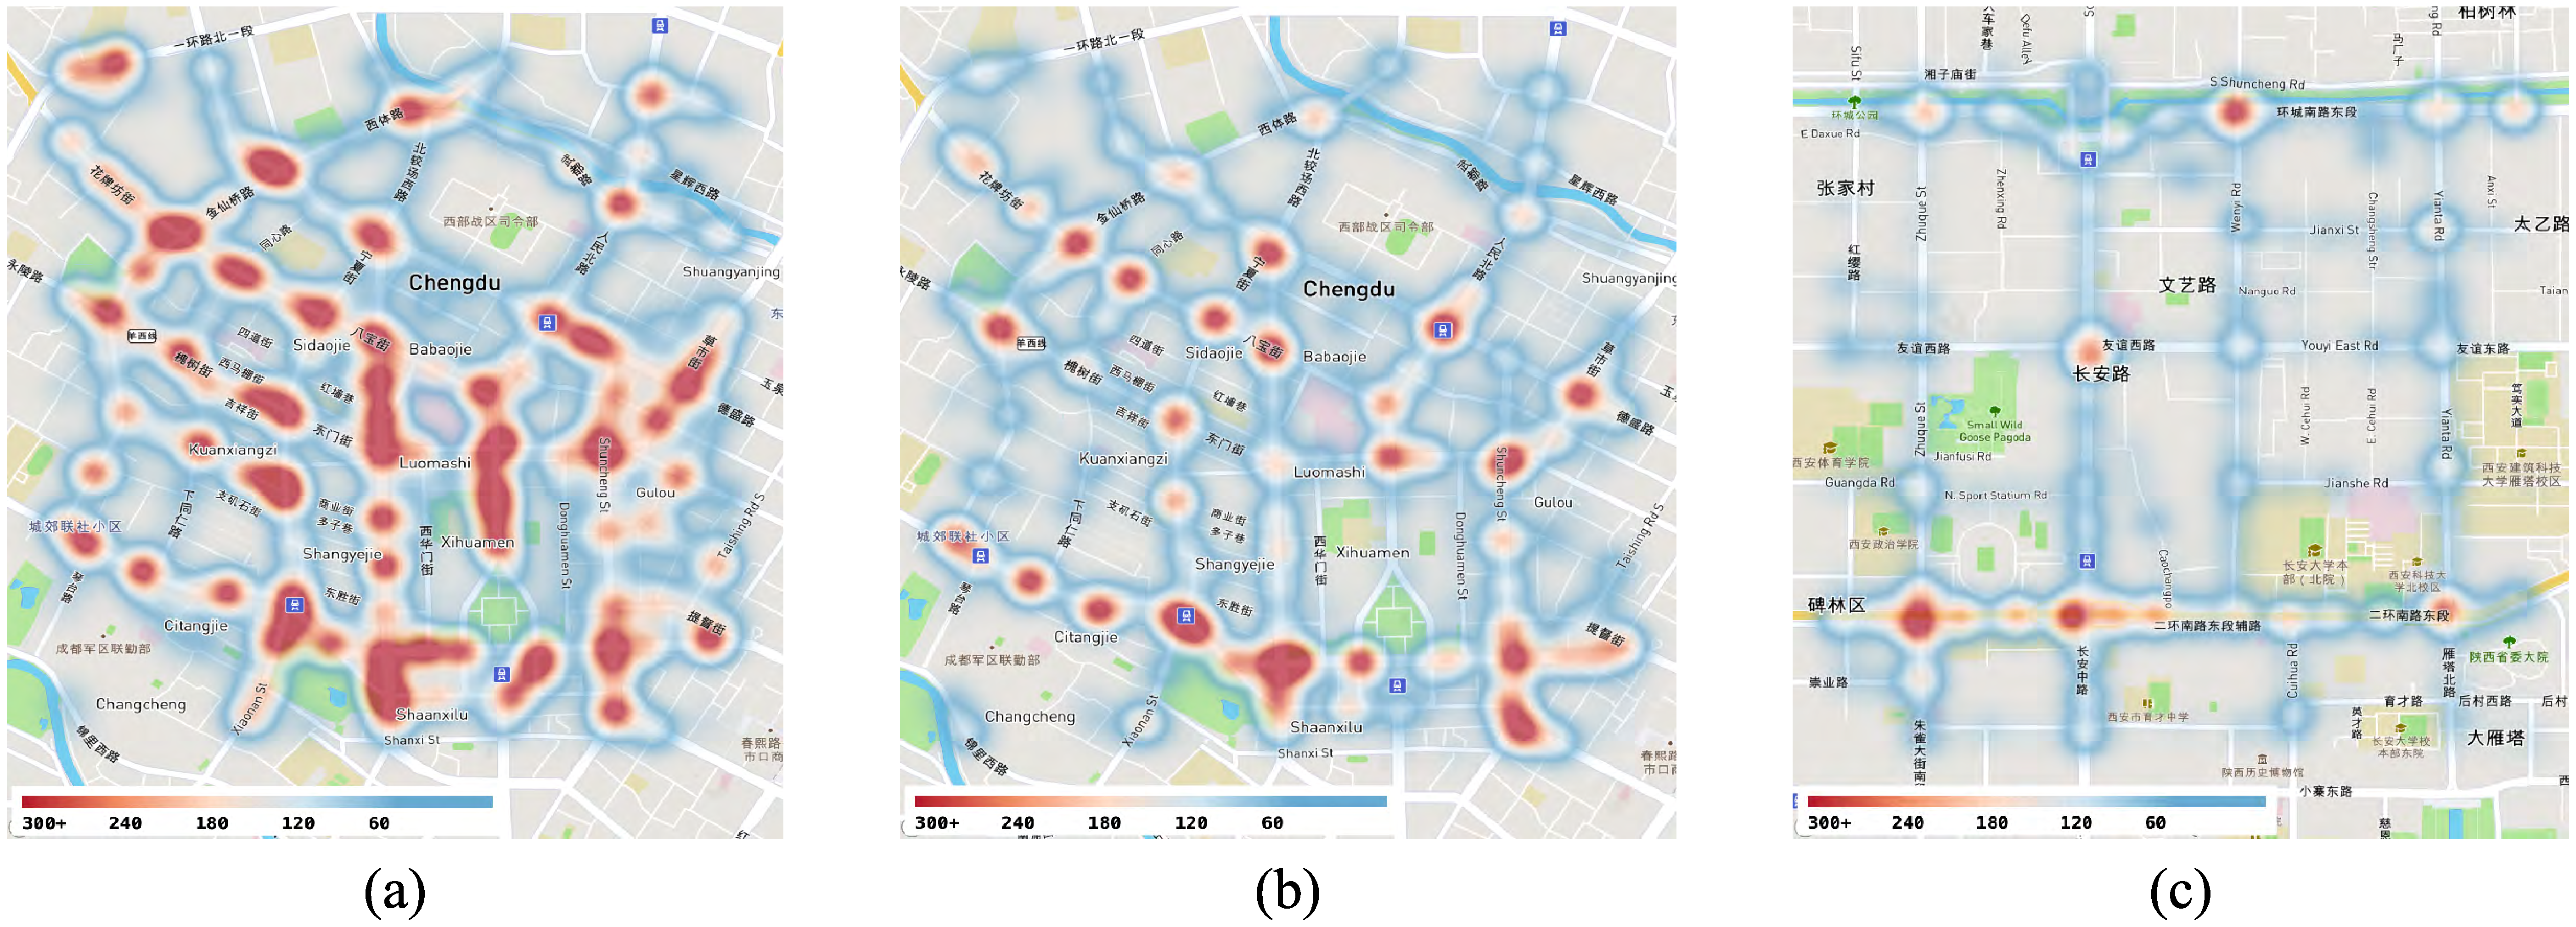
\includegraphics[width=1\columnwidth]{Fig2-5-heat-map.pdf}
  \bicaption[不同场景下的车辆分布热力图]{不同场景下的车辆分布热力图。(a) 场景1(b)场景2(c)场景3}[Heat map of the distribution of vehicles under different scenarios]{Heat map of the distribution of vehicles under different scenarios. (a) Scenario 1 (b) Scenario 2 (c) Scenario 3}
  \label{fig 2-5}
\end{figure} 

MADR的架构和超参数描述如下:
本地行动者网络是一个四层全连接的神经网络,其中包含两个隐藏层,其神经元数量分别为64和32。
目标行动者网络结构与本地行动者网络相同。
本地评论家网络是一个四层全连接的神经网络,其中包含两个隐藏层,其神经元数量分别为128和64。
目标评论家网络的结构与本地评论家网络相同。
使用整流线性单元(Rectified Linear Unit, ReLU)作为激活函数,使用自适应矩估计(Adaptive Moment Estimation, Adam)优化器更新网络权重,本地行动者网络和本地评论家网络学习率均为 0.001,奖励折扣因子为 0.996。
经验回放缓存$|\mathcal{B}|$的大小为100000,批大小为512。
此外,本章还实现了以下四种可比较的算法。

\begin{itemize}
	\item \textbf{随机分配}: 在每个时间片中,随机选择一个关于确定感知频率、上传优先级和V2I带宽分配的动作。
	\item \textbf{集中式深度确定性策略梯度}\cite{mlika2022deep}: 在边缘节点实现一个智能体,根据系统状态以集中的方式确定感知频率、上传优先级和V2I带宽分配。同时,智能体接收系统奖励以评估其贡献。
	\item \textbf{多智能体行动者-评论家}\cite{he2021efficient}: 实现了车辆中的智能体,基于本地车联网环境观测来决定感知频率和上传优先级,以及边缘节点中的智能体来决定V2I带宽分配。每个智能体都接收相同的系统奖励以评估其贡献。
	\item \textbf{采用VBA策略的多智能体行动者-评论家}: 为了更好地分配V2I带宽,本章进一步设计了一个多智能体行动者-评论家算法的变体,其中边缘节点基于VBA策略来分配V2I带宽,其余部分与MAAC算法一致。
\end{itemize}

此外,本章还设计了以下指标用于性能评估。
\begin{itemize}
	\item \textbf{累积奖励} (Cumulative Reward, CR): 定义为调度期间的累积系统奖励, 其计算方法为:
		\begin{equation}
			\operatorname{CR} = \sum_{\forall t \in \mathbf{T}} r\left(\boldsymbol{a}_{v}^{t},\boldsymbol{a}_{e}^{t} \mid \boldsymbol{o}^{t}\right)
		\end{equation}
	\item \textbf{平均奖励的构成} (Composition of Average Reward, CAR): 定义为归一化的时效性、完整性和一致性在平均奖励中的百分比,其表示为:
		\begin{equation}
			\operatorname{CAR} \triangleq <\frac{3}{10}(1-\hat{\Xi}_{i}),\frac{4}{10}(1-\hat{\Phi}_{i}), \frac{3}{10}(1-\hat{\Psi}_{i})>
		\end{equation}
	\item \textbf{平均排队时间} (Average Queuing Time, AQT): 定义为感知信息的排队时间之和除以调度期$T$内的信息数量,其计算方法为:
		\begin{equation}
			\operatorname{AQT} =\sum_{\forall t \in \mathbf{T}} \left \{ \frac{\sum_{v \in \mathbf{V}} \sum_{\forall d \subseteq \mathbf{D}_{v}^t} \frac{\operatorname{q}_{d, v}^t}{|\mathbf{D}_{v}^t|} }{V} \right\} \bigg/ T
		\end{equation}
	\item \textbf{服务率} (Service Ratio, SR): 定义为满足完整性要求的视图的数量在调度期间$\mathbf{T}$所需的视图总数的占比,其计算方法是:
		\begin{equation}
			\operatorname{SR} = \frac{\sum_{\forall t \in \mathbf{T}}\sum_{\forall i \in \mathbf{I}_e^t} \mathds{1}\{\Phi_{i} \geq \Phi_{th}\}}{ \sum_{\forall t \in \mathbf{T}} |\mathbf{I}_e^t|}
		\end{equation}
	其中 $\Phi_{th}$ 是完整性阈值。
\end{itemize}

\subsection{实验结果与分析}

\textbf{1) 算法收敛性:}
图\ref{fig 2-6}比较了五种算法在收敛速度和CR值方面的表现。结果显示,本章提出的MADR算法收敛速度最快(约660次迭代),并获得了最高的CR值(约357)。相比之下,C-DDPG、MAAC和MAAC-VBA分别需要大约4500次、950次和870次迭代才能收敛,并分别达到约307、290和315的CR值。RA作为基线算法的CR值约为241。值得注意的是,与C-DDPG、MAAC和MAAC-VBA相比,MADR算法在CR值方面分别实现了大约16.3\%、23.1\%和13.3\%的增加,同时在收敛速度方面分别提升了大约6.8倍、1.4倍和1.3倍。这主要是因为MADR算法旨在维护车辆的稳定通信环境,从而使车辆中的行动者和评论家网络的训练更加有效。另外,由于MADR的动作空间较小,相比于C-DDPG,MADR更容易收敛,因为C-DDPG需要同时决定感知频率、上传优先级和V2I带宽分配。

\begin{figure}[h]
\centering
  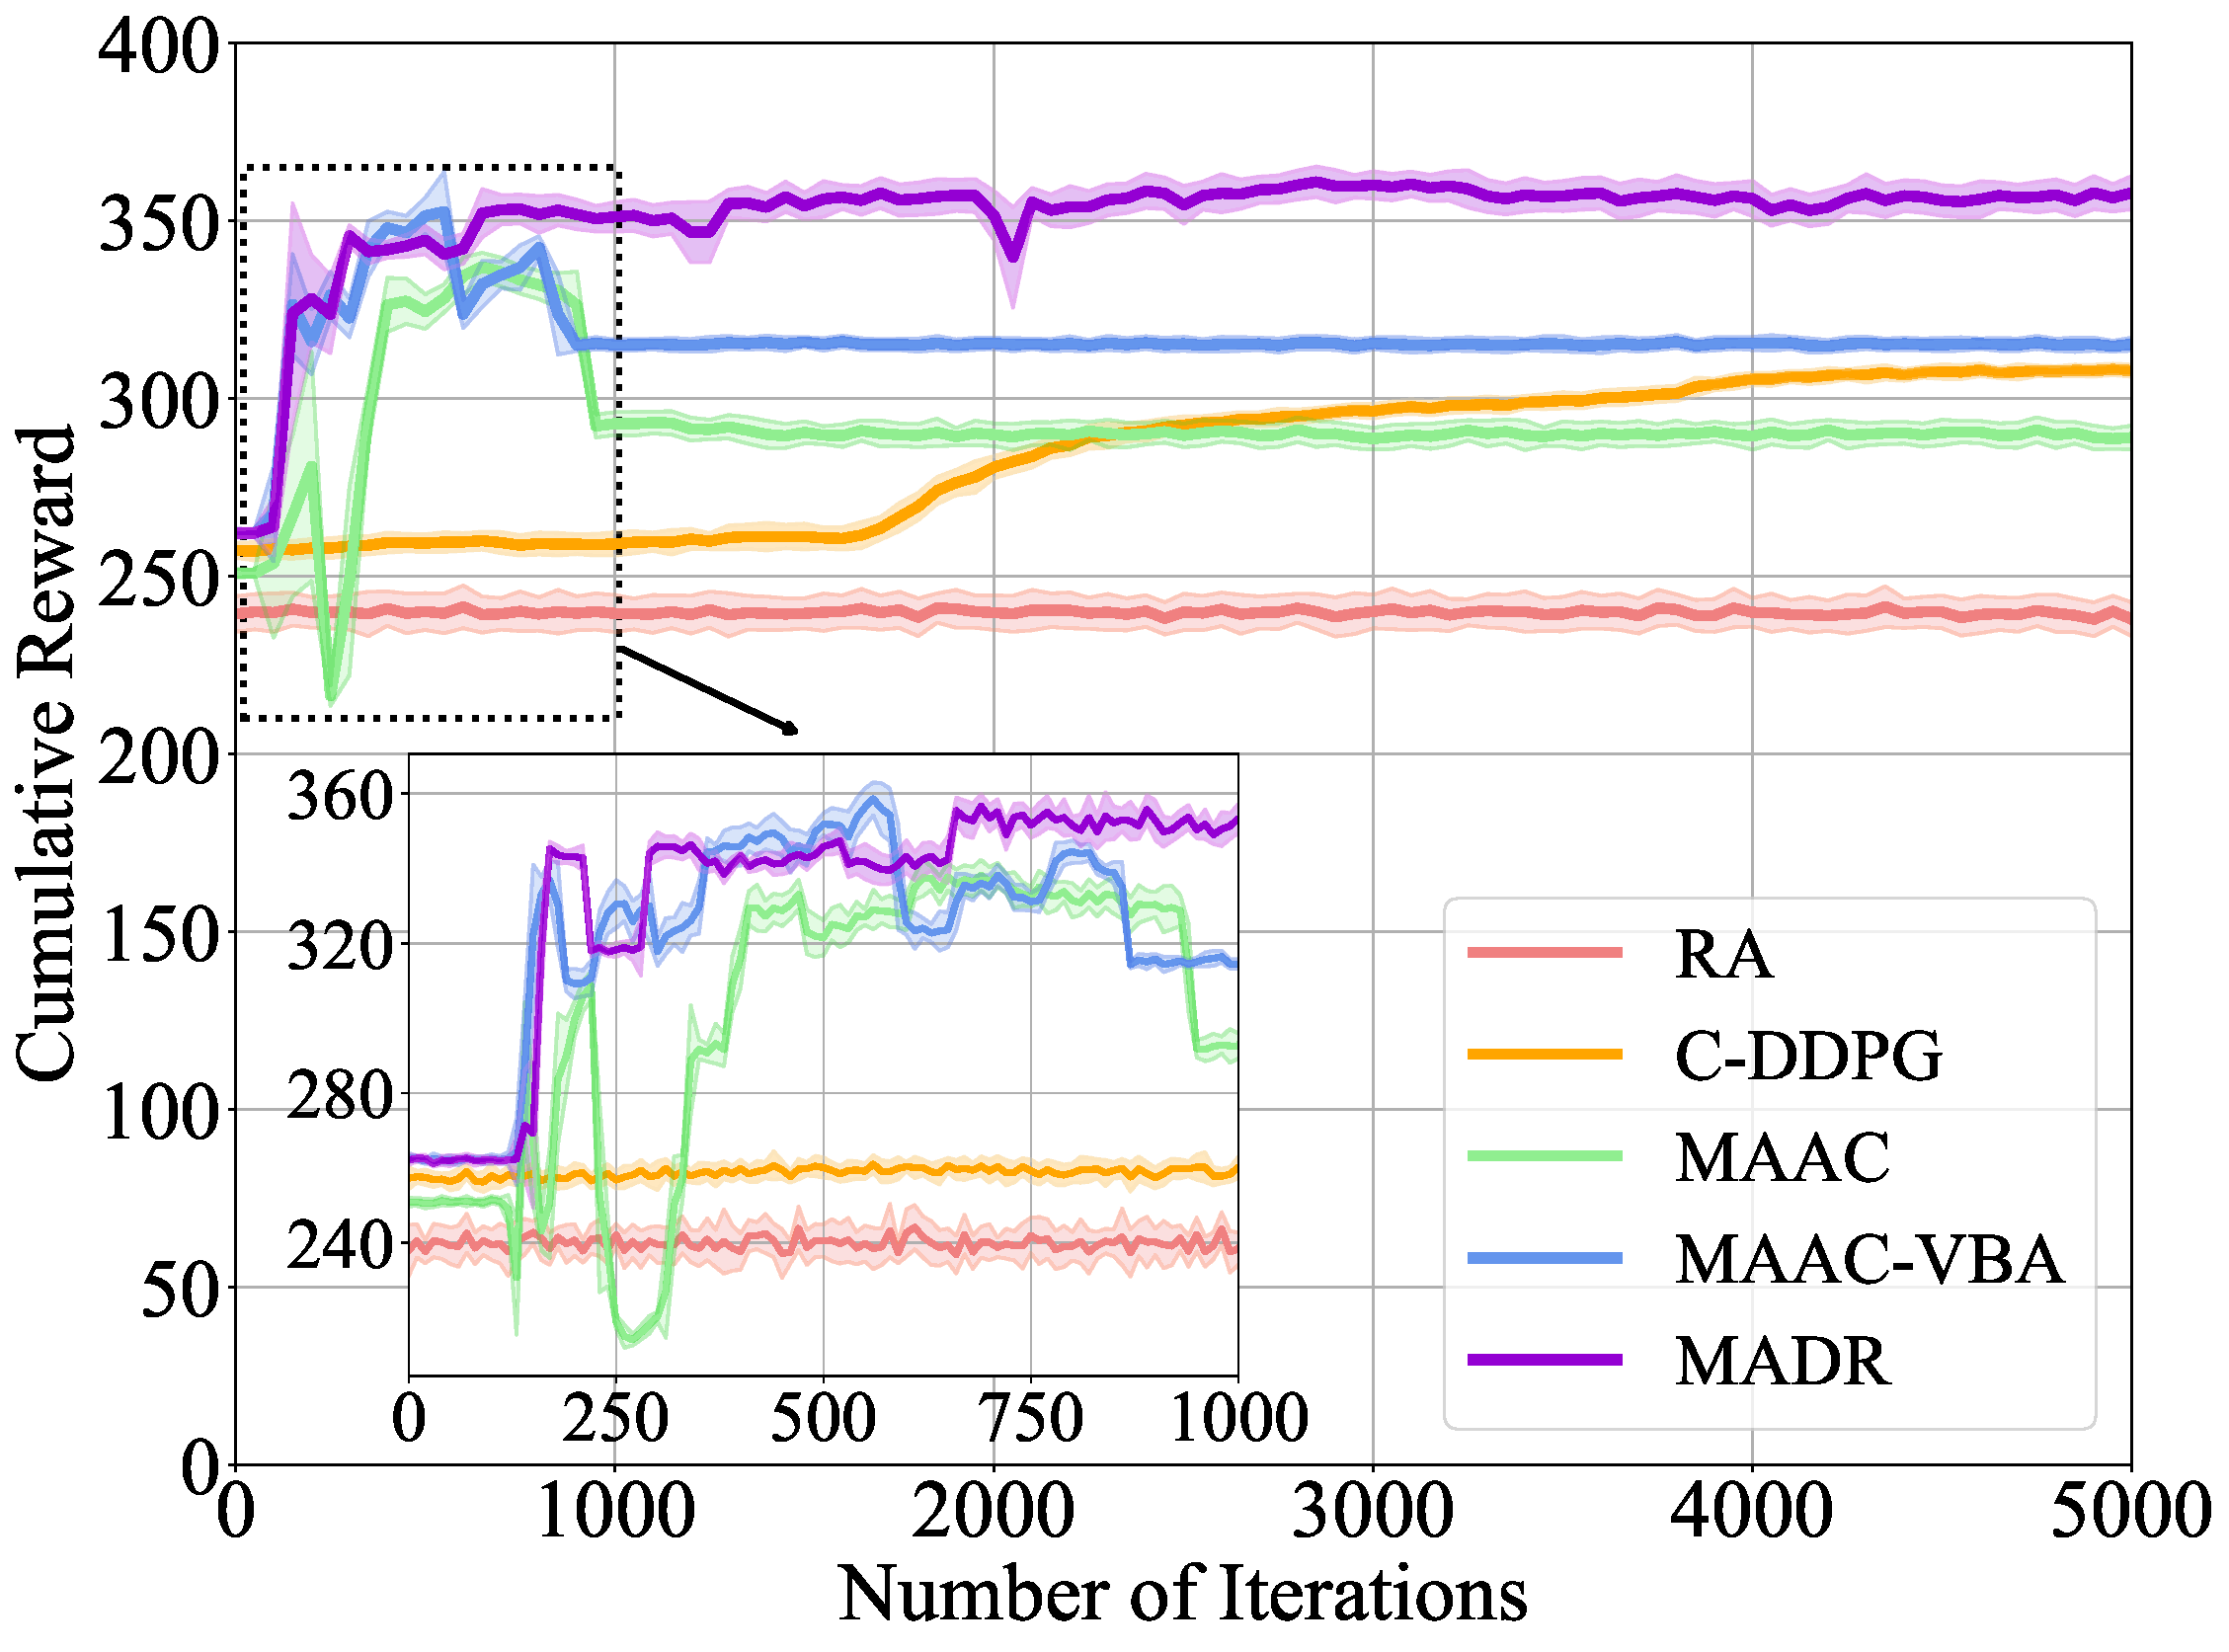
\includegraphics[width=0.75\columnwidth]{Fig2-6-convergence.pdf}
  \bicaption{算法收敛性比较}{Convergence comparison}
  \label{fig 2-6}
\end{figure} 

\begin{figure}[h]
  \centering
  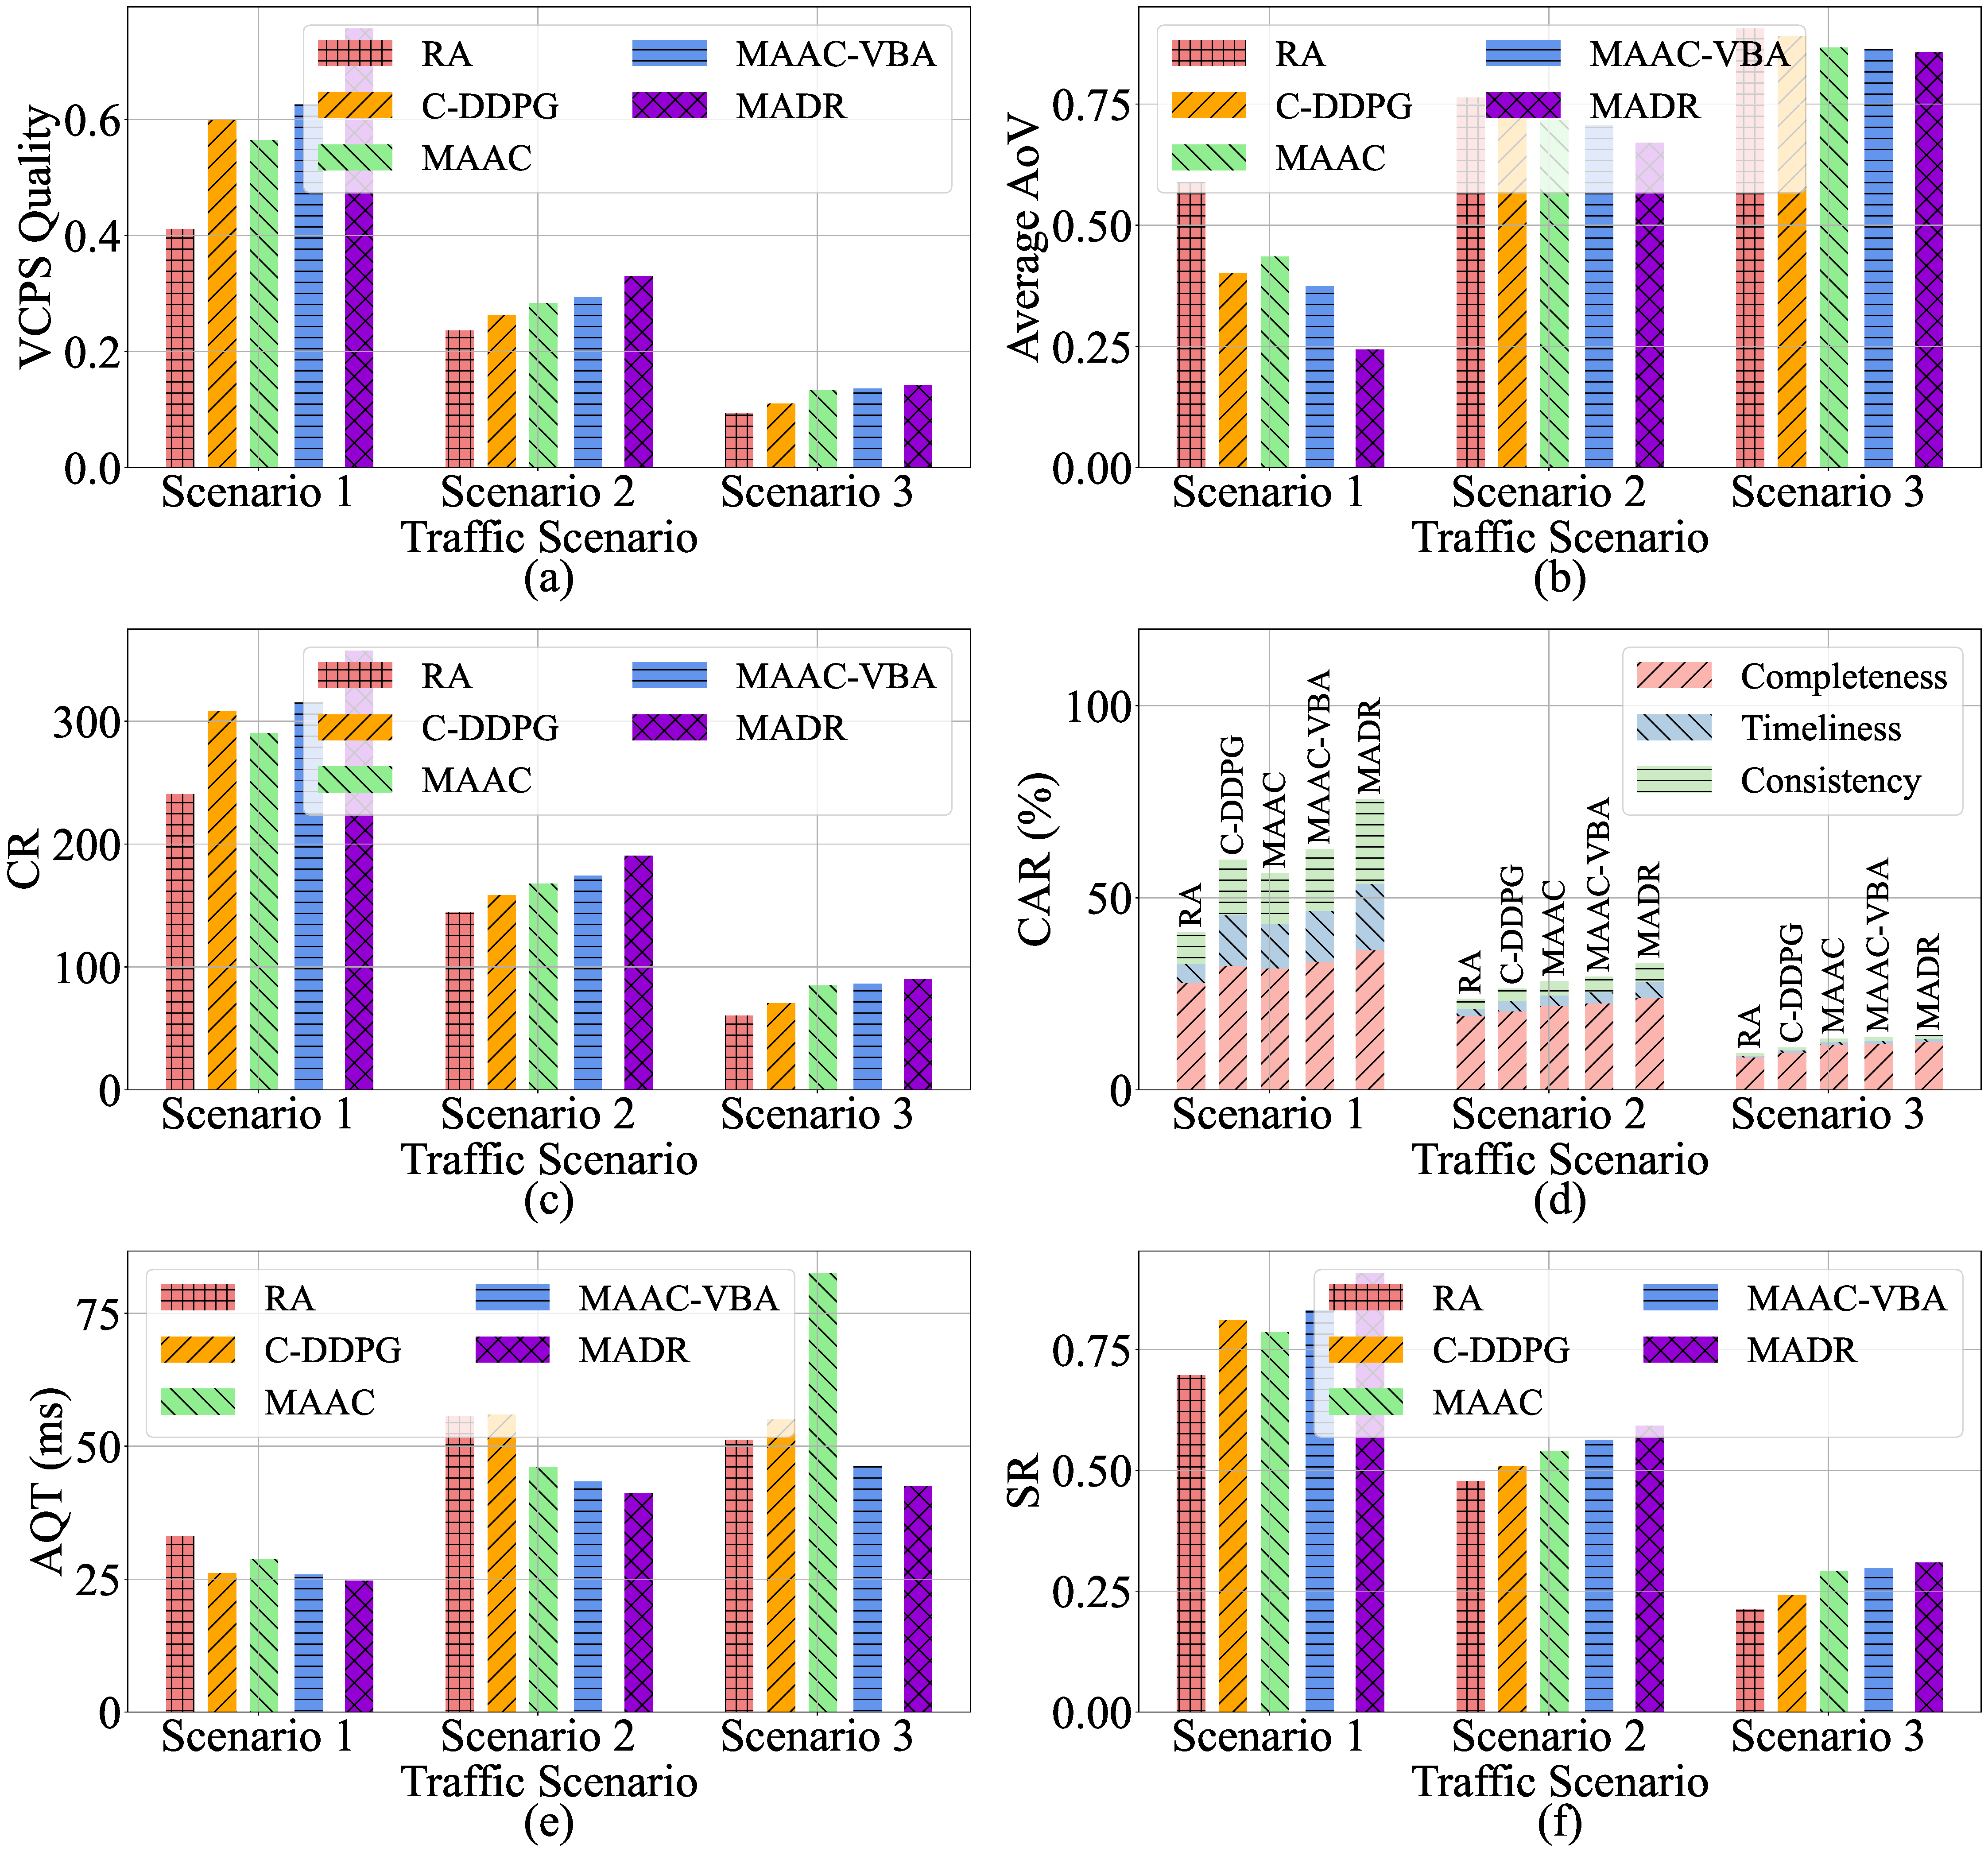
\includegraphics[width=1\columnwidth]{Fig2-7-different-scenarios.pdf}
  \bicaption[不同交通场景下的性能比较]{不同交通场景下的性能比较。(a)车载信息物理融合系统质量(b)平均 AoV(c)累积奖励(d)平均奖励的构成(e)平均排队时间(f)服务率}[Performance comparison under different traffic scenarios]{Performance comparison under different traffic scenarios. (a) Vehicular cyber-physical system quality (b) Average age of view (c) Cumulative reward (d) Composition of average reward (e) Average queuing time (f) Service ratio}
  \label{fig 2-7}
\end{figure}

\textbf{2) 交通场景的影响:}
图\ref{fig 2-7}比较了五种算法在不同交通场景下的表现。图\ref{fig 2-7}(a) 显示了五种算法在VCPS质量方面的比较。如图所示,MADR算法在所有场景下都实现了最高的VCPS质量,比RA、C-DDPG、MAAC和MAAC-VBA分别平均提高了58.0\%、27.1\%、19.1\%和12.5\%的VCPS质量。图\ref{fig 2-7}(b) 显示了五种算法在平均AoV方面的比较。所有场景下,MADR都实现了最低的平均AoV。图\ref{fig 2-7}(c) 显示了五种算法在CR方面的比较。结果表明,MADR实现的CR高于RA、C-DDPG、MAAC和MAAC-VBA。在场景3下,MADR和MAAC-VBA的CR相似,原因是场景3中较低的车辆密度和较高的车辆动态性使得数据上传比场景1和2中更加困难。图\ref{fig 2-7}(d) 将平均奖励分解成时效性、完整性和一致性三个部分的比例,以显示五种算法在这些方面的表现。在场景3下,时效性和一致性都非常小,这主要是因为当视图不完整时,时效性和一致性的要求很难得到满足。图\ref{fig 2-7}(e) 和图\ref{fig 2-7}(f) 显示了五种算法在不同场景下的AQT和SR比较。结果表明,MADR实现了最低的AQT,并在所有场景下保持最高的SR。

\begin{figure}[h]
  \centering
  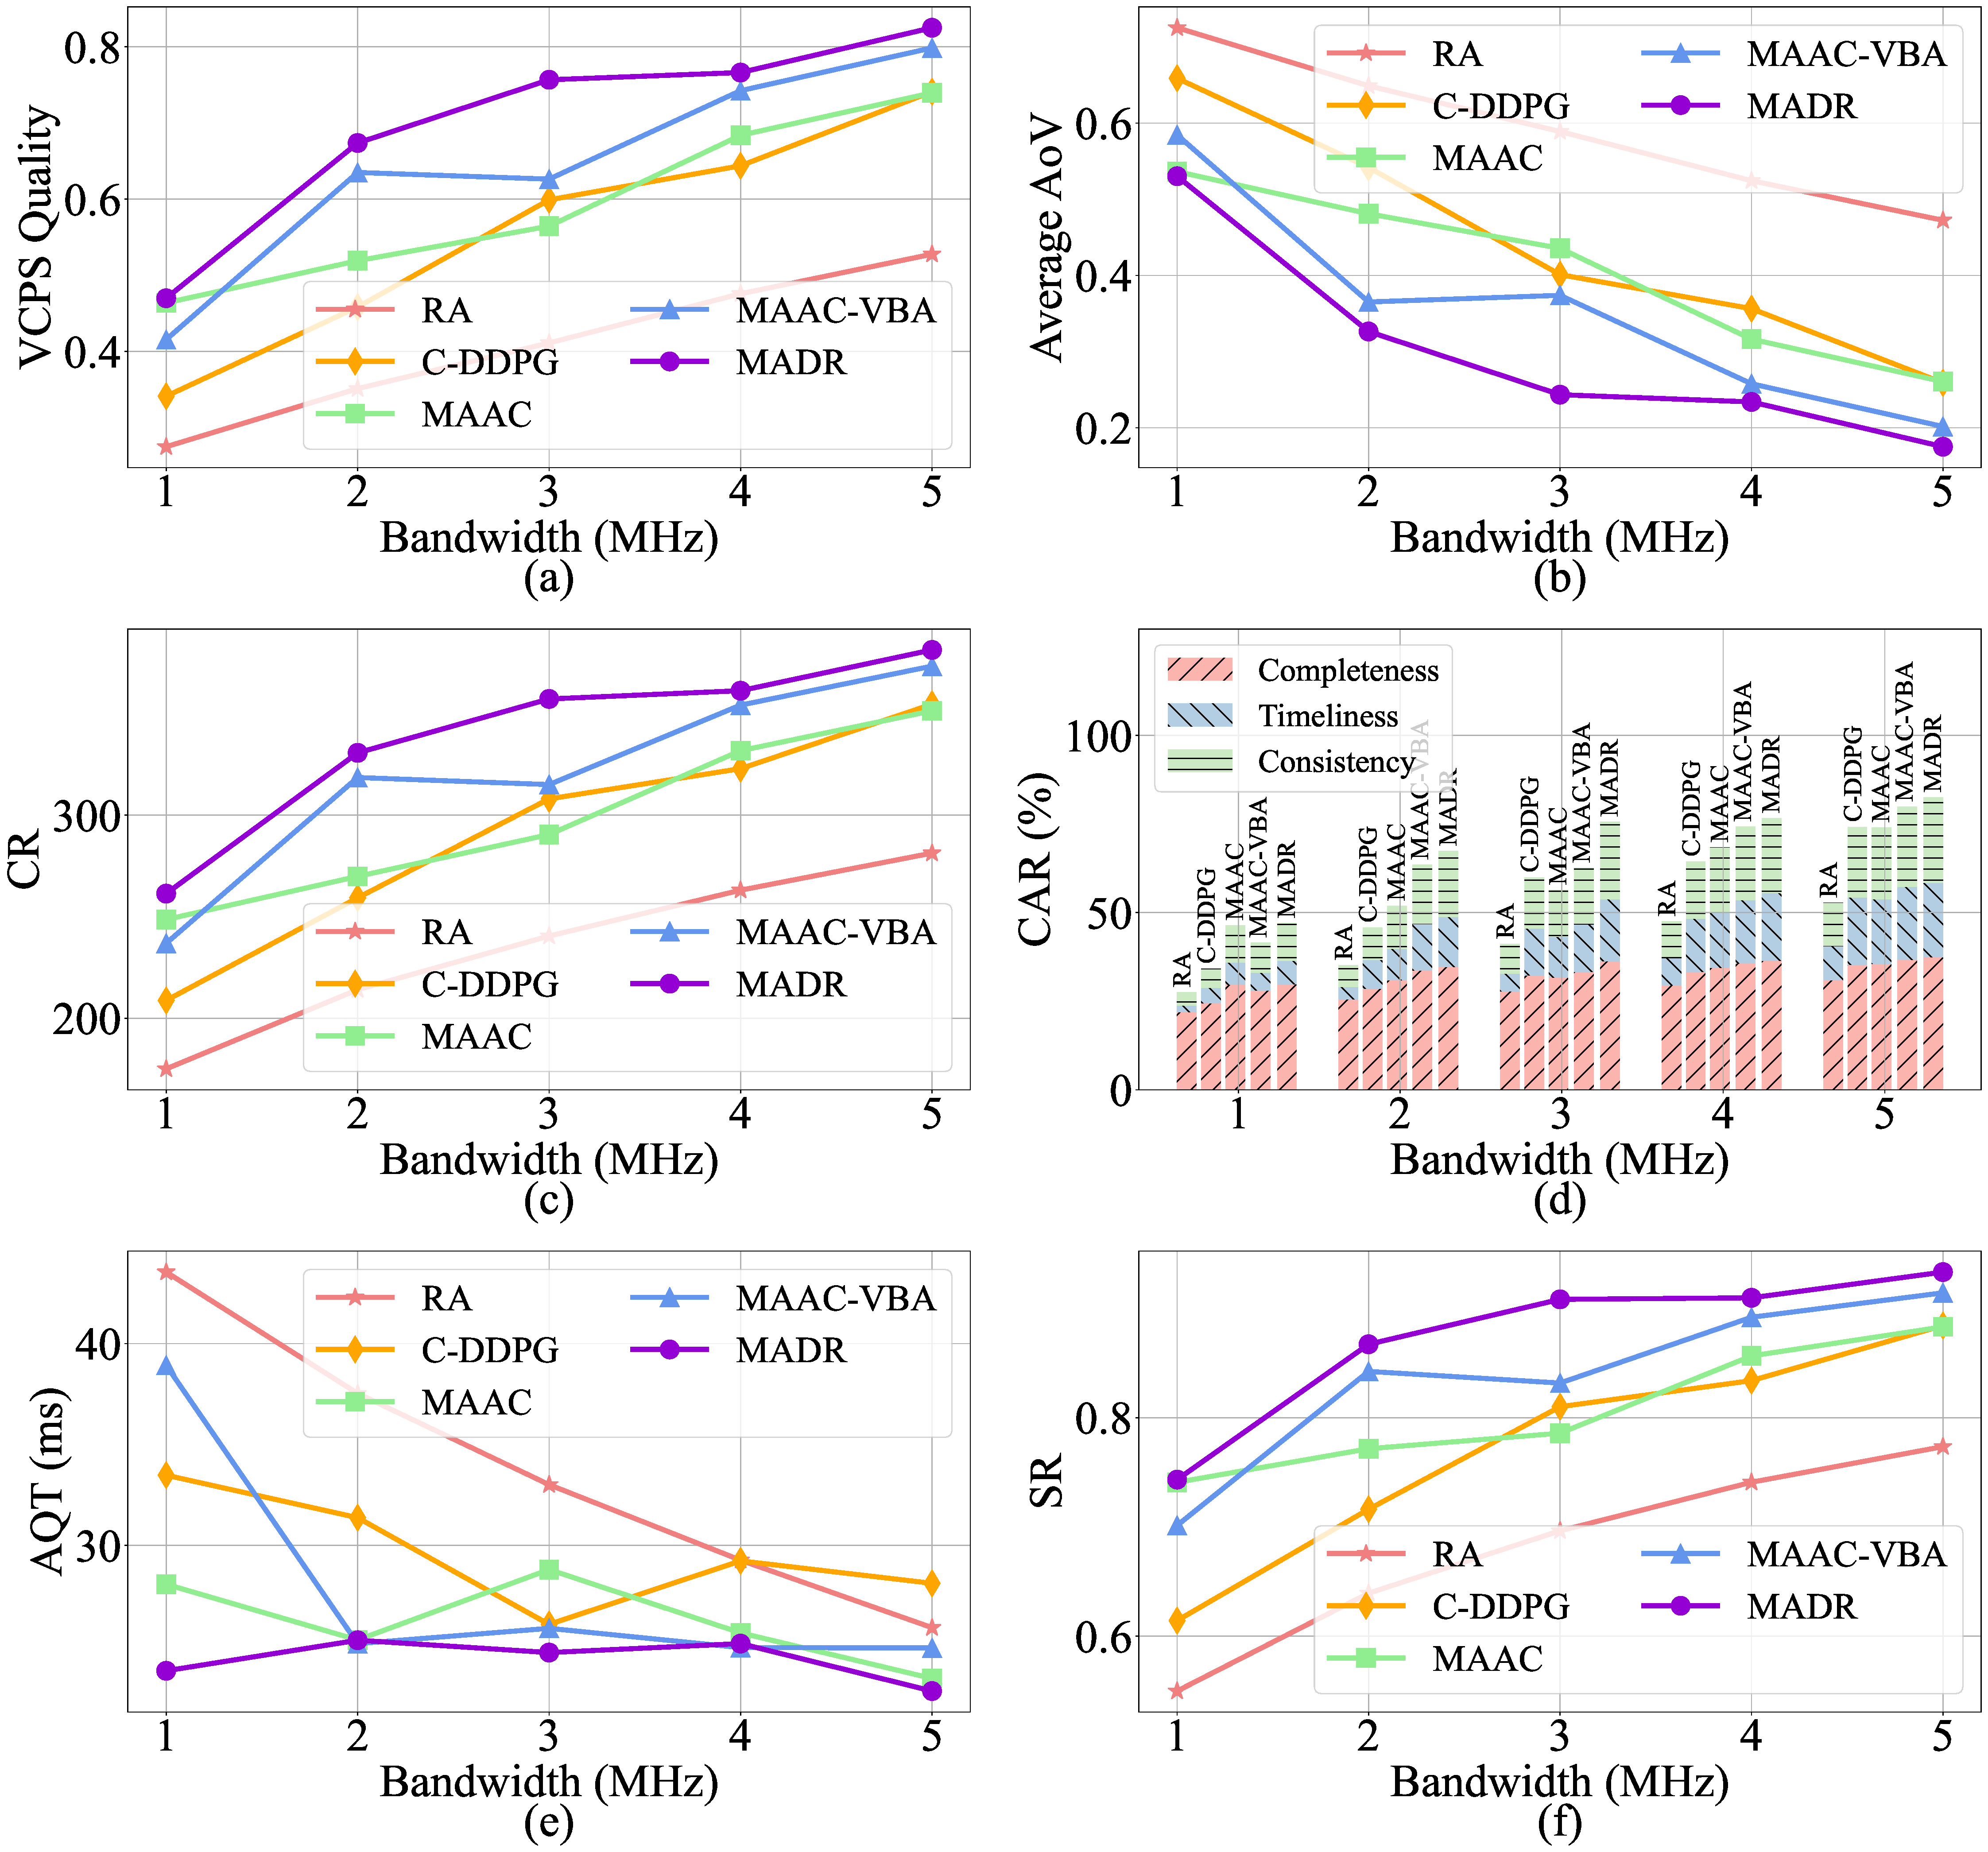
\includegraphics[width=1\columnwidth]{Fig2-8-different-bandwidths.pdf}
  \bicaption[不同V2I带宽下的性能比较]{不同V2I带宽下的性能比较。(a)车载信息物理融合系统质量(b)平均 AoV(c)累积奖励(d)平均奖励的构成(e)平均排队时间(f)服务率}[Performance comparison under different V2I bandwidths]{Performance comparison under different V2I bandwidths. (a) Vehicular cyber-physical system quality (b) Average age of view (c) Cumulative reward (d) Composition of average reward (e) Average queuing time (f) Service ratio}
  \label{fig 2-8}
\end{figure}

\textbf{3) V2I 带宽的影响:}
图\ref{fig 2-8}比较了不同V2I带宽下五种算法的性能。在这组实验中,边缘节点的V2I带宽从1 MHz增加到5 MHz,更大的带宽代表更多的信息可以通过V2I通信上传。图\ref{fig 2-8}(a) 显示了五种算法在VCPS质量方面的比较。随着带宽的增加,所有算法的VCPS质量都相应增加。在不同V2I带宽下,MADR的VCPS质量分别比RA、C-DDPG、MAAC和MAAC-VBA高出约72.9\%、28.3\%、17.8\%和9.3\%。图\ref{fig 2-8}(b) 显示了五种算法在平均AoV方面的比较。所有情况下,MADR实现了最低的平均AoV。图\ref{fig 2-8}(c) 显示了五种算法在CR方面的比较。当带宽增加时,所有五种算法的性能都有所提升。具体来说,相比于RA、C-DDPG、MAAC和MAAC-VBA,MADR在CR方面分别实现了75.1\%、29.4\%、22.7\%和10.6\%的提升。图\ref{fig 2-8}(d) 比较了五种算法在CAR方面的表现。MADR比其他四种算法表现更好,特别是在视图时效性和一致性方面。这是因为在有限的带宽下,所提出的方案中车辆之间的信息感知和上传的协作更加有效。图\ref{fig 2-8}(e) 显示了五种算法在AQT方面的比较。在不同的V2I带宽下,MADR的AQT保持最低,反映了MADR能够更有效地分配带宽。图\ref{fig 2-8}(f) 显示了五种算法在SR方面的比较。在所有情况下,MADR的SR都保持最高水平,进一步证明了MADR在利用有限带宽方面的优势。

\begin{figure}[h]
  \centering
  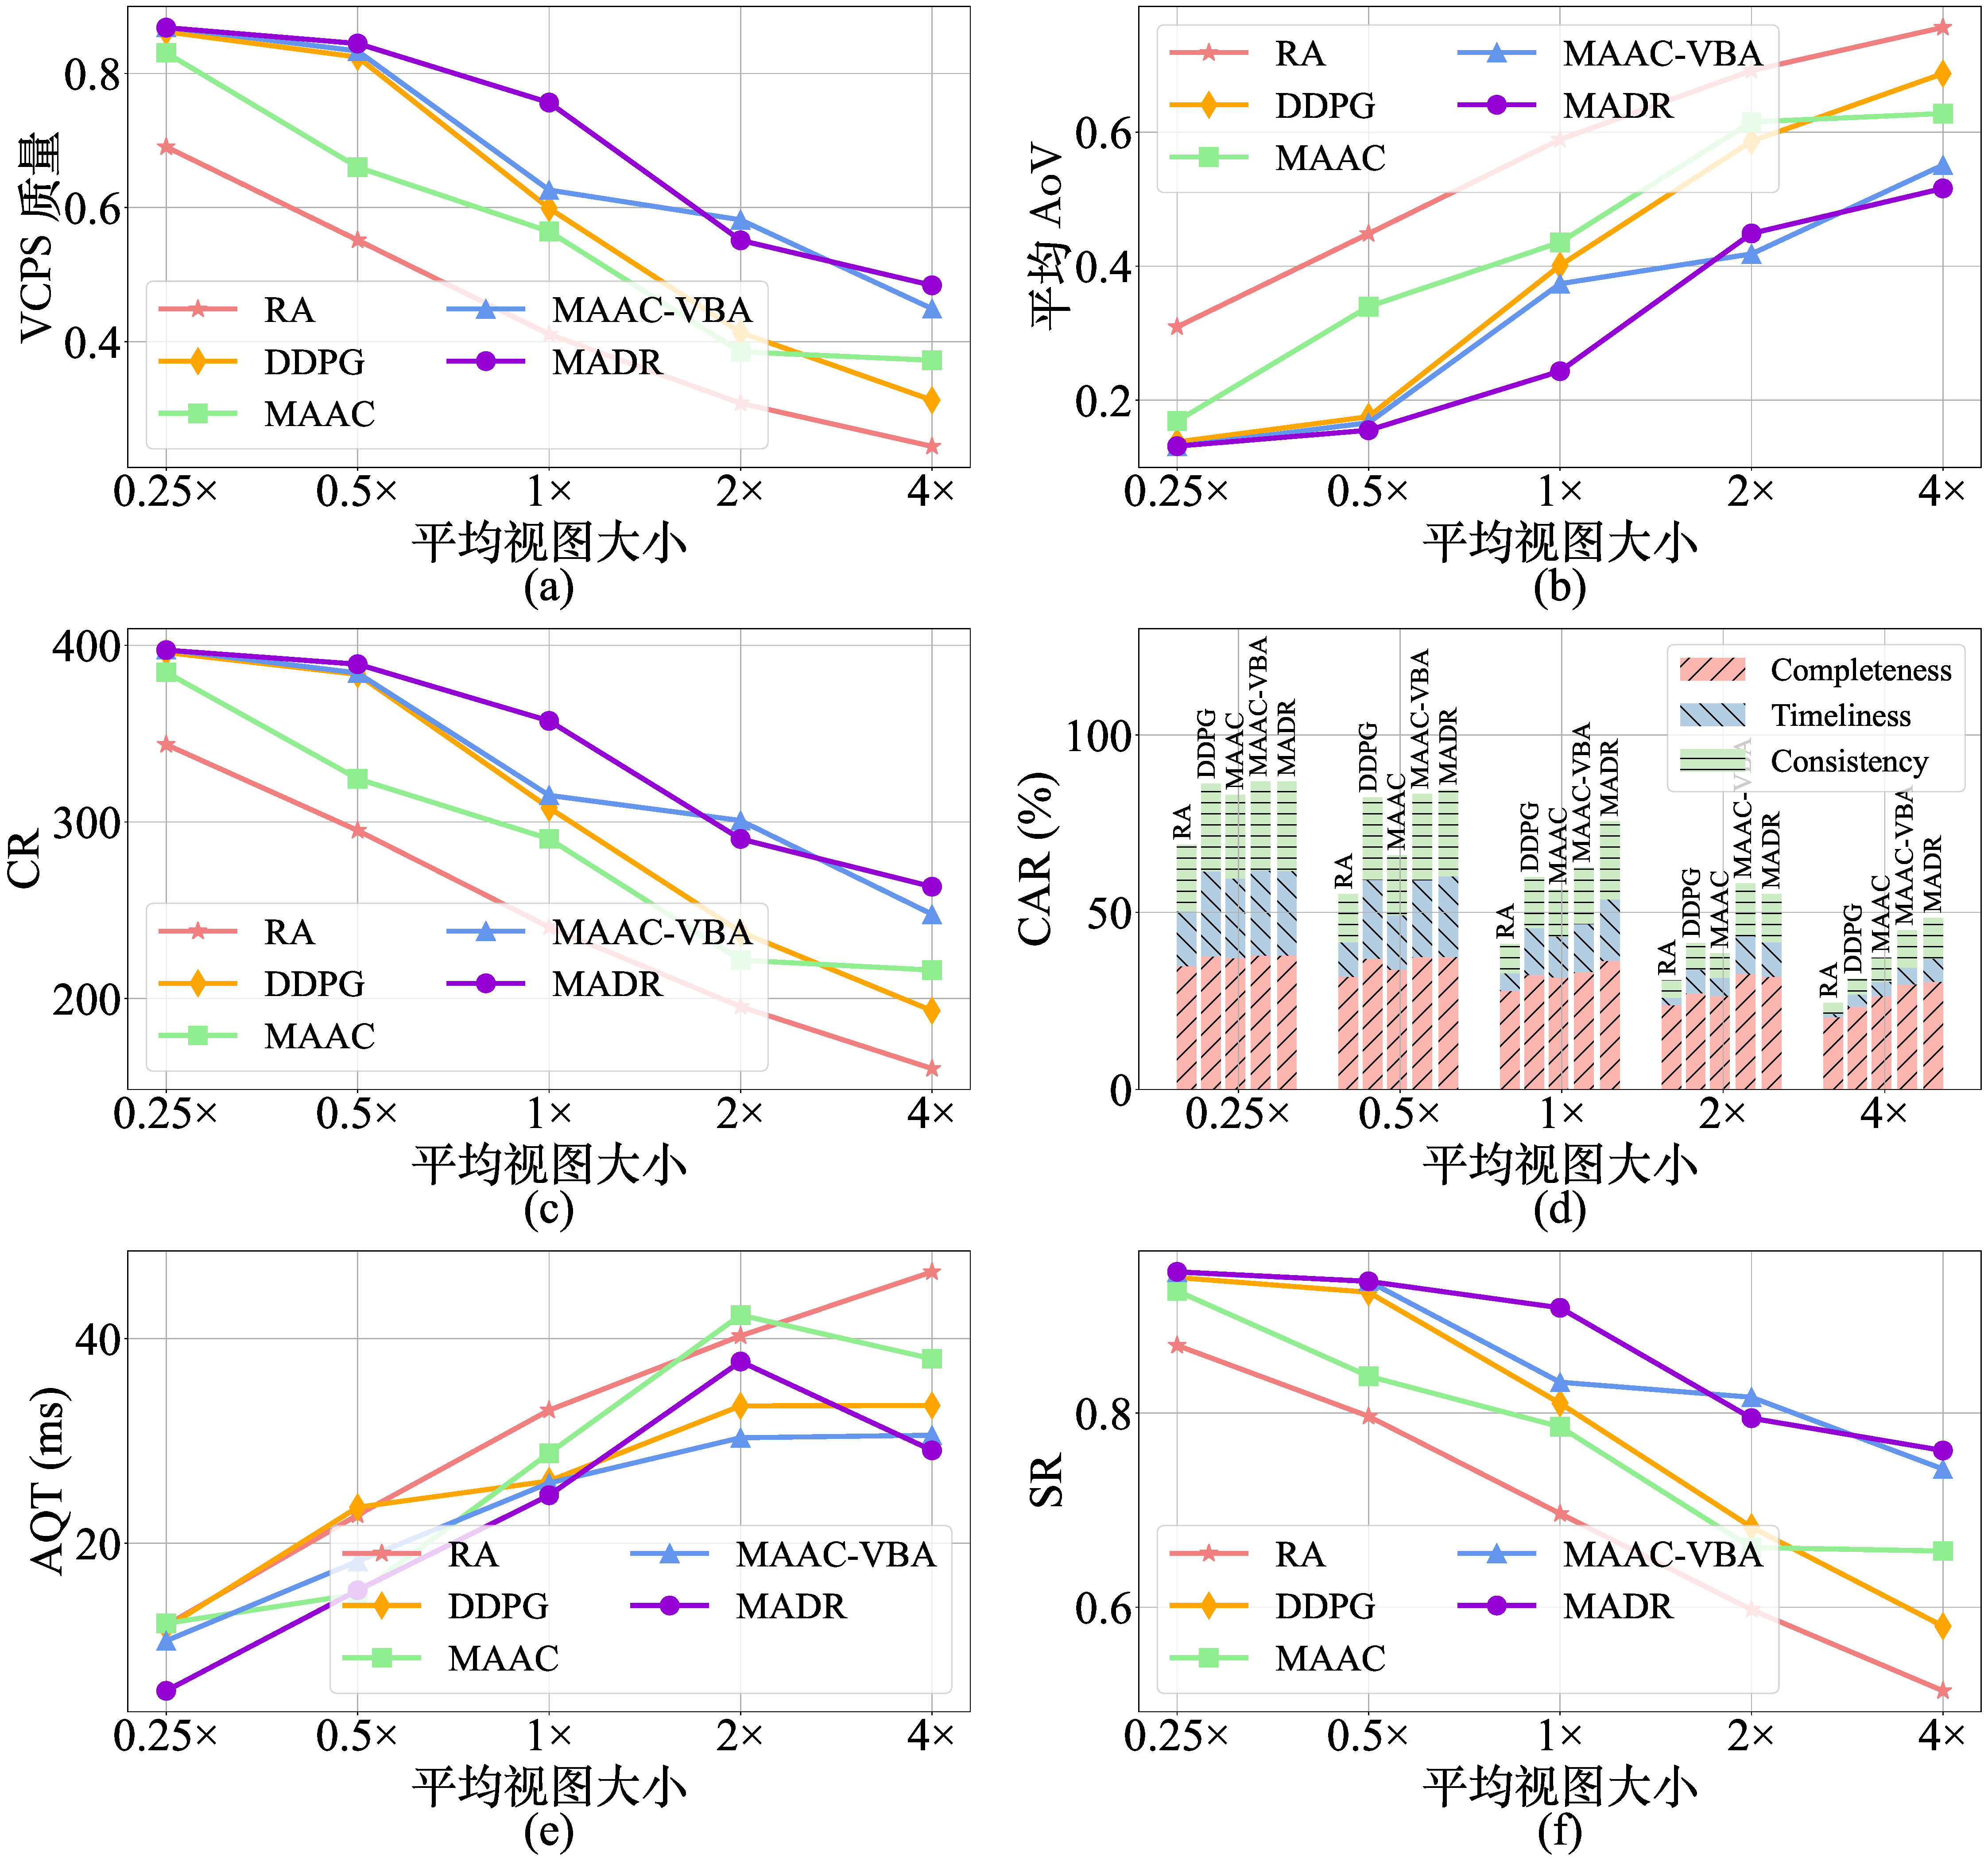
\includegraphics[width=1\columnwidth]{Fig2-9-different-view-sizes.pdf}
  \bicaption[不同视图需求下的性能比较]{不同视图需求下的性能比较。(a)车载信息物理融合系统质量(b)平均 AoV(c)累积奖励(d)平均奖励的构成(e)平均排队时间(f)服务率}[Performance comparison under different requirements on views]{Performance comparison under different requirements on views. (a) Vehicular cyber-physical system quality (b) Average age of view (c) Cumulative reward (d) Composition of average reward (e) Average queuing time (f) Service ratio}
  \label{fig 2-9}
\end{figure}

\textbf{4) 视图需求的影响:}
图\ref{fig 2-9}比较了五种算法在不同视图需求下的性能,其中ITS应用需求的视图平均大小从0.25倍增加到4倍,作为基准,1倍视图的平均大小约为6.46 MB。图\ref{fig 2-9}(a) 显示了五种算法在VCPS质量方面的比较。随着平均视图大小的增加,所有算法的性能都会变差。在不同的视图需求下,MADR在最大限度地提高VCPS质量方面分别比RA、C-DDPG、MAAC和MAAC-VBA高出约68.1\%、23.5\%、27.9\% 和4.9\%。图\ref{fig 2-9}(b)和图\ref{fig 2-9}(c) 比较了五种算法在平均AoV和CR方面的表现。当平均视图大小较小时,MADR中的平均AoV略低于MAAC和MAAC-VBA。MADR、MAAC和MAAC-VBA的CR相似,因为较小的数据量有较高的成功上传的概率。图\ref{fig 2-9}(d) 比较了五种算法在CAR方面的表现。当平均视图大小从0.25倍增加到0.5倍时,MADR和MAAC-VBA之间的性能差异较小,原因是当有足够的资源来满足较小的平均视图大小的要求时,算法的调度效果并不明显。图\ref{fig 2-9}(e) 和图\ref{fig 2-9}(f) 显示了五种算法在AQT和SR方面的比较。结果表明,MADR可以保持最低的AQT,同时在大多数情况下实现最高的SR。当平均视图大小为2倍时,MAAC-VBA实现了最低的AQT和最高的SR,这反映了所提出的VBA方案可以更有效地分配带宽。

\section{本章小结}\label{section 2-7}

本章设计了一个包括应用层、控制层、虚拟层和数据层的车联网分层服务架构,以最大化软件定义网络和移动边缘计算范式的协同效应。
在此基础上,本章提出了分布式感知与异质信息融合场景,并考虑了车载信息物理融合中异质信息的时效性、完整性和一致性,设计了质量指标AoV用于评估边缘构建的逻辑视图。
形式化定义了最大化VCPS质量的问题,并设计了一个基于差分奖励的多智能体深度强化学习解决方案,其中车辆作为独立智能体,决定感知频率和上传优先级。
边缘节点基于车辆预测轨迹和视图需求,通过VBA策略分配V2I带宽。
并采用基于DR的信用分配方案,根据车辆差分奖励评估其对于视图构建的贡献。
通过仿真实验的全面性能评估表明,MADR算法比RA、C-DDPG、MAAC和MAAC-VBA在最大限度地提高VCPS质量方面分别高出约61.8\%、23.8\%、22.0\%和8.0\%,同时加快了收敛速度。